\documentclass[12pt,a4paper]{article}

% ---------------------------------------------------------------- packages
\usepackage[T1]{fontenc}
\usepackage[utf8]{inputenc}
\usepackage{mathptmx}                 % Times, as in the Faculty's sample papers
\usepackage[a4paper,left=3cm,right=2.5cm,top=2.5cm,bottom=2.5cm]{geometry}
\usepackage{setspace}\setstretch{1.3}
\usepackage{amsmath,amssymb}
\usepackage{graphicx}
\usepackage{booktabs,tabularx,multirow,array}
\usepackage{float}
\usepackage[labelfont=bf,font=small]{caption}
\usepackage{subcaption}
\usepackage{enumitem}\setlist{itemsep=2pt,topsep=4pt}
\usepackage{xcolor}
\usepackage{listings}
\usepackage{tikz}
\usetikzlibrary{arrows.meta,positioning,fit,calc}
\usepackage[numbers,sort&compress]{natbib}
\usepackage{xurl}
\usepackage[hidelinks]{hyperref}
\usepackage{microtype}
\usepackage{titlesec}
\titleformat{\section}{\Large\bfseries}{\thesection}{1em}{}
\titleformat{\subsection}{\large\bfseries}{\thesubsection}{1em}{}
\titleformat{\subsubsection}{\normalsize\bfseries}{\thesubsubsection}{1em}{}
\setlength{\parindent}{1.5em}
\setlength{\parskip}{2pt}

\definecolor{codebg}{HTML}{F5F5F2}
\lstset{basicstyle=\ttfamily\footnotesize,backgroundcolor=\color{codebg},frame=single,rulecolor=\color{gray!40},
  breaklines=true,columns=fullflexible,keepspaces=true,showstringspaces=false,xleftmargin=4pt,xrightmargin=4pt}

\newcommand{\code}[1]{\texttt{\small #1}}
\renewcommand{\bibname}{Bibliography}

\begin{document}

% ---------------------------------------------------------------- cover
\begin{titlepage}
\centering
\vspace*{5cm}
{\LARGE\bfseries BSc THESIS\par}
\vspace{6cm}
\hfill{\large Qudrat Ullah}\par
\vfill
{\large Debrecen\\2026\par}
\end{titlepage}

% ---------------------------------------------------------------- title page
\begin{titlepage}
\centering
{\large\bfseries University of Debrecen\\Faculty of Informatics\\Department of Data Science and Visualization\par}
\vspace{3.2cm}
{\LARGE\bfseries A Hybrid Multimodal Lab Assistant: Blood Image Classification Combined with Domain-Expert LLM Reasoning and RAG\par}
\vfill
\begin{minipage}[t]{0.48\textwidth}
\raggedright
\textbf{Supervisor:}\\
Dr.\ András Hajdu\\
Professor
\end{minipage}\hfill
\begin{minipage}[t]{0.48\textwidth}
\raggedleft
\textbf{Candidate:}\\
Qudrat Ullah\\
Computer Science BSc
\end{minipage}
\vspace{2cm}

{\itshape ``I consent to the submission of this work for review.''\par}
\vspace{2cm}
{\large Debrecen\\2026\par}
\end{titlepage}

% ---------------------------------------------------------------- contents
\pagenumbering{arabic}
\setcounter{page}{1}
\tableofcontents
\clearpage

\section{Introduction}

This thesis was written on the topic \emph{Development of a domain expert using a large language model like ChatGPT}. Large language models (LLMs) of the GPT-4 class answer many medical questions at the level of a well-read student \cite{singhal2023}, so it is tempting to use such a model directly as an ``expert''. In a clinical field, however, a general-purpose model has three weaknesses: it can produce fluent but unsupported claims (hallucination \cite{ji2023}); it offers no provenance, and may even invent references that do not exist \cite{walters2023}; and it has no access to the case --- here, the cells on a blood-smear image --- so its answers are generic. In this thesis, a \emph{domain expert} is therefore an LLM-based system that answers within one field, grounds its statements in curated domain literature and cites it, inspects case-specific evidence through tools, and signals when a human expert must take over.

\paragraph{Choice of application.} The topic is addressed through a concrete system: a \emph{hybrid multimodal lab assistant} for peripheral blood smears. The blood smear is one of the most informative tests in hematology: a stained drop of blood is examined under the microscope, and the proportions of the white-cell types (the \emph{differential}) can reveal infection, leukaemia or bone-marrow disease. Manual review is slow and observer-dependent, which has motivated much work on automated cell classification \cite{acevedo2019,habibzadeh2018}; but such systems stop at a label per cell. Turning the labels into a clinical interpretation requires domain knowledge. Hematology is therefore a natural test bed for an LLM domain expert, because it combines visual, case-specific evidence, which image models can extract, with textbook knowledge, which the expert must supply.

\paragraph{Theoretical and practical importance.} Theoretically, the thesis compares the main ways of turning a general LLM into a domain expert --- retrieval-augmented generation (RAG), tool use and parameter-efficient fine-tuning --- on the same domain, and asks what each of them actually contributes. Practically, it shows how such an expert can be connected to image analysis in a way that is inspectable and safe: every automated finding carries an uncertainty estimate, every claim can be traced to a retrieved source, and the decision to involve a human is taken by explicit rules rather than by the model. It also examines whether an open model that can run on local hardware can replace a commercial API, which matters wherever patient data may not leave the institution.

\subsection{Aims and research questions}

The aim is to build and evaluate the lab assistant and, through it, to answer four research questions:

\begin{description}[leftmargin=1.2cm,style=nextline]
  \item[RQ1] Can standard deep-learning models (YOLOv8, EfficientNet-B0) detect and classify blood cells accurately and attach a useful uncertainty estimate and a saliency map to every classified white cell?
  \item[RQ2] How can a general-purpose LLM be turned into a hematology domain expert with retrieval-augmented generation and domain-specific tools, and what does the resulting assistant produce on real smear images?
  \item[RQ3] Does QLoRA fine-tuning of an open-weight model (Llama-3.1-8B-Instruct) on textbook-grounded question--answer pairs improve its hematology answers compared with the same model without fine-tuning?
  \item[RQ4] Can the combined system make its reasoning inspectable and hand difficult cases to a human through deterministic rules --- and where does this fail?
\end{description}

\subsection{Research methods}

The work combines system development with quantitative evaluation. The image-analysis stages were trained on public benchmark datasets (TXL-PBC for detection, PBC for classification) and evaluated on held-out test sets with standard metrics, complemented by a calibration and error-detection analysis of the uncertainty estimate. The domain expert was built from a knowledge base of 1{,}049 textbook passages, a GPT-4o agent with five hematology tools, and a Llama-3.1-8B model fine-tuned with QLoRA on synthetic question--answer pairs generated from the same textbooks. The fine-tuned model was compared with its base version and with GPT-4o on held-out questions (similarity to reference answers and ratings by an LLM judge) and on external exam questions, using paired statistical tests. Finally, a complete run of the assistant was analysed as a case study. All code, notebooks, configuration and results are part of the submitted software artefact.

The main findings, detailed in Chapter~\ref{sec:results}, are that the image models perform strongly on the benchmark data (98.60\,\% classification accuracy, with uncertainty scores that detect errors with an AUROC of 0.97), and that fine-tuning changed \emph{how} the open model answers --- closer to the textbook, without invented citations --- but not \emph{what} it knows: its clinical correctness did not improve, and GPT-4o remained the most correct system. Knowledge and provenance therefore have to come from retrieval, and safety from explicit rules.

\subsection{Structure of the thesis}

Chapter~\ref{sec:background} reviews how domain-expert LLMs are built and the related work on blood-smear analysis, uncertainty and interpretability. Chapter~\ref{sec:data} describes the data and knowledge sources, and Chapter~\ref{sec:arch} the architecture of the lab assistant. Chapter~\ref{sec:method} gives the training procedures and the evaluation protocol, and Chapter~\ref{sec:results} presents and discusses the results, including the case study and the limitations. Chapter~\ref{sec:conclusion} concludes and outlines future work.

\clearpage

\section{Theoretical Background}\label{sec:background}

\subsection{Large language models and their limits in medicine}

A large language model is a transformer network trained to predict the next token of text on a very large corpus and then further trained to follow instructions and hold a dialogue. Models such as GPT-4o \cite{openai2024gpt4o} and the open-weight Llama~3 family \cite{grattafiori2024llama3} can answer questions, summarise documents and produce structured output such as JSON. Singhal \emph{et al.} showed that instruction-tuned LLMs encode a substantial amount of clinical knowledge and can answer medical exam questions at a high level \cite{singhal2023}.

The same work, and a large literature on hallucination \cite{ji2023}, also shows the limits. An LLM generates the most plausible continuation of a text, not the most correct one. When its internal knowledge is incomplete it may produce a confident but false statement, and when asked for references it may produce citations that look real but do not exist \cite{walters2023}. The model also has no access to information outside its prompt, so it cannot know the data of a specific patient unless that data is given to it. For a clinical assistant these are serious problems: a fluent wrong answer is more dangerous than no answer, because it is more likely to be believed.

\subsection{Building domain experts from general LLMs}\label{sec:bg-expert}

There are three main ways to make a general LLM behave as an expert in a narrow field. They are complementary, and this thesis uses all three (Table~\ref{tab:approaches}).

\paragraph{Prompting.} The cheapest approach is a carefully written system prompt (``You are a clinical hematology expert\ldots''), together with rules and an output format. Prompting changes the style and focus of the answers, but it does not add knowledge the model lacks, it does not provide sources, and it does not prevent unsupported statements.

\paragraph{Retrieval-augmented generation (RAG).} RAG \cite{lewis2020} leaves the model unchanged and supplies relevant passages from a curated corpus at question time. The source documents are split into chunks, each chunk is converted into a vector by a sentence-embedding model \cite{reimers2019}, and the vectors are stored in a vector database. For each question, the chunks whose vectors are most similar to the question's vector are retrieved and placed in the prompt, together with an instruction to answer from them and to cite them. RAG has two important properties for a domain expert: the knowledge can be updated without retraining, and every answer can be checked against the passages it was based on. Comparative studies have found retrieval to be more reliable than fine-tuning for injecting new factual knowledge into an LLM \cite{ovadia2024}.

\paragraph{Domain fine-tuning.} Fine-tuning changes the model's weights using examples from the domain. Medical models such as Med-PaLM \cite{singhal2023} and Meditron \cite{chen2023meditron} were built this way, but full fine-tuning of a model with billions of parameters is too expensive for most projects. \emph{Parameter-efficient} methods solve this. LoRA \cite{hu2022lora} freezes the original weight matrices $W$ and learns a low-rank update, so that a layer computes
\begin{equation}
  h = W x + \frac{\alpha}{r}\, B A x, \qquad B \in \mathbb{R}^{d \times r},\ A \in \mathbb{R}^{r \times k},\ r \ll \min(d,k),
\end{equation}
where only $A$ and $B$ are trained. QLoRA \cite{dettmers2023qlora} additionally stores the frozen model in 4-bit precision, which makes it possible to fine-tune an 8-billion-parameter model on a single 16\,GB GPU such as the free NVIDIA T4 in Google Colab. Fine-tuning is particularly effective at teaching \emph{behaviour}: answer length and structure, terminology, citation format and cautious phrasing. It also produces an open model that can be run on local hardware, independent of a commercial API.

\paragraph{Synthetic training data.} When no suitable human-written training data exist, question--answer pairs can be generated by a stronger model from trusted source text, in the spirit of Self-Instruct \cite{wang2023selfinstruct}. This is fast and cheap, but the generated data inherit the generator's mistakes and style, which must be considered when the resulting model is evaluated.

\begin{table}[H]
\centering
\caption{Ways of turning a general LLM into a domain expert, and how this thesis uses them.}
\label{tab:approaches}
\small
\begin{tabularx}{\textwidth}{l X X X}
\toprule
 & \textbf{Adds knowledge?} & \textbf{Gives checkable sources?} & \textbf{Role in this thesis} \\
\midrule
Prompting & No & No & System prompts and JSON output schema \\
RAG & Yes, at query time & Yes, retrieved passages & Textbook knowledge base (Sec.~\ref{sec:kb}) \\
Fine-tuning (QLoRA) & Mostly style and behaviour & No (model may imitate a citation format) & Open, self-hostable expert (Sec.~\ref{sec:ft}) \\
Tools / agent & Yes, case data and reference values & Yes, logged tool calls & GPT-4o ReAct agent (Sec.~\ref{sec:agent}) \\
\bottomrule
\end{tabularx}
\end{table}

\subsection{Tool use and the ReAct agent paradigm}

Standard RAG performs one retrieval followed by one generation. ReAct \cite{yao2023react} generalises this by interleaving reasoning and acting: the model writes a thought, chooses an action (a call to a tool), observes the result, and repeats until it produces a final answer. Tools can be database searches, calculators or reference tables. For a domain expert this has two advantages. The model can look up exact reference values and case data instead of relying on memory, and every tool call is recorded, so the path to the final answer can be audited. LangGraph \cite{langgraph} provides an implementation of this loop with structured tool calling, which is used in this thesis.

\subsection{Evaluating a domain expert}

A domain expert can be evaluated in three complementary ways:
\begin{enumerate}
  \item \textbf{Multiple-choice questions} with known answers, such as the medical entrance-exam questions of MedMCQA \cite{pal2022medmcqa}. They give an objective accuracy, but test recognition of facts rather than explanation.
  \item \textbf{Similarity of free-text answers to reference answers}, measured by word overlap (ROUGE-L, based on the longest common subsequence \cite{lin2004rouge}) or by the cosine similarity of sentence embeddings. These measures are cheap and reproducible, but they reward answers that \emph{look like} the reference, not necessarily answers that are correct.
  \item \textbf{Graded judgements} of answers by clinicians or, more cheaply, by a strong LLM used as a judge \cite{zheng2023judge}. An LLM judge scales well but has its own biases and does not replace expert review.
\end{enumerate}
This thesis uses the first two, and inspects answers qualitatively (Section~\ref{sec:eval}).

\subsection{Automated peripheral blood-smear analysis}

Image-based analysers for blood smears have existed since the 2000s, first with classical image processing and later with deep learning. Acevedo \emph{et al.} showed that convolutional neural networks can classify single blood-cell images with very high accuracy \cite{acevedo2019} and published the PBC dataset of 17{,}092 cell images in eight classes, recorded with a CellaVision DM96 analyser \cite{acevedo2020}. For locating cells in a whole field of view, general object detectors of the YOLO family \cite{jocher2023yolov8} are fine-tuned on annotated smears such as BCCD \cite{mooney2018bccd} and the more recent TXL-PBC collection \cite{gan2024txlpbc}.

Most of this work stops at a label per cell; the interpretation of the differential as a whole is left to the human reader. Table~\ref{tab:related} places the present system among typical approaches. The comparison is qualitative: it describes capabilities of system families, not of every individual system.

\begin{table}[H]
\centering
\caption{Qualitative comparison of system families.}
\label{tab:related}
\footnotesize
\begin{tabularx}{\textwidth}{>{\raggedright\arraybackslash}p{2.6cm} X X X X}
\toprule
\textbf{System family} & \textbf{Image analysis} & \textbf{Uncertainty} & \textbf{Explanation} & \textbf{Clinical interpretation} \\
\midrule
General LLM chat (e.g.\ ChatGPT) & None (text only) & None & Free text, no sources & Generic, not case-specific \\
CNN cell classifiers & Pre-cropped cells & Usually softmax only & Rare or post-hoc & None \\
Detector + classifier pipelines & Detection and classification & Rarely passed on & Boxes, sometimes saliency & None \\
\textbf{This thesis} & YOLOv8s + EfficientNet-B0 & MC-Dropout level per cell, review flag & Boxes, Grad-CAM, citations, tool trace & RAG + tool-using LLM expert; QLoRA open model \\
\bottomrule
\end{tabularx}
\end{table}

\subsection{Uncertainty and explainability}

A neural network's softmax output is not a calibrated probability; modern networks tend to be over-confident \cite{guo2017}. Bayesian deep learning treats the network weights as random variables, but exact inference is intractable. Practical approximations include deep ensembles \cite{lakshminarayanan2017}, which train several networks and average them, and \emph{Monte Carlo Dropout} \cite{gal2016}, which keeps dropout active at prediction time and averages $T$ stochastic forward passes. MC-Dropout needs no retraining when the network already contains dropout layers, which is why it is used here; its disadvantage is that it is only an approximation and is usually less well calibrated than ensembles.

Grad-CAM \cite{selvaraju2017} produces a heatmap showing which image regions most influenced a class prediction. It weights the feature maps $A^k$ of a convolutional layer by the average gradient of the class score $y^c$:
\begin{equation}
  L^c_{\text{Grad-CAM}} = \mathrm{ReLU}\Big(\sum_k \alpha_k^c A^k\Big), \qquad \alpha_k^c = \frac{1}{Z}\sum_{i,j}\frac{\partial y^c}{\partial A^k_{ij}}.
\end{equation}
In a clinical setting Grad-CAM is most useful as a check: if the heatmap highlights the background or a neighbouring cell rather than the cell of interest, the prediction should be treated as suspect.

\subsection{Trustworthy AI in medical decision support}

Regulatory and policy documents --- the FDA's Good Machine Learning Practice principles \cite{fda2021gmlp}, the EU Artificial Intelligence Act \cite{euaiact2024} and the WHO guidance on large multi-modal models in health \cite{who2024lmm} --- converge on a few requirements for high-risk medical AI: transparency about inputs and limits, auditability of decisions, communication of uncertainty, and effective human oversight. These requirements guided the design of the system in this thesis. The system is a research prototype: it is not clinically validated, not a medical device, and not intended for use on patient data outside a research setting.

\clearpage

\section{Data and Knowledge Sources}\label{sec:data}

The system uses five data sources: two for the domain expert's knowledge, one for evaluating it externally, and two for training the vision models that provide case evidence (Table~\ref{tab:datasets}).

\begin{table}[H]
\centering
\caption{Data sources used in the thesis.}
\label{tab:datasets}
\small
\begin{tabularx}{\textwidth}{>{\raggedright\arraybackslash}p{3.4cm} X >{\raggedright\arraybackslash}p{3.8cm}}
\toprule
\textbf{Source} & \textbf{Content} & \textbf{Used for} \\
\midrule
Hematology textbooks \cite{kawthalkar2006,schmaier2012} & 541 PDF pages, 1{,}049 text chunks & RAG knowledge base; source of Q\&A pairs \\
Synthetic hematology Q\&A & 2{,}098 question--answer pairs generated from the chunks & Fine-tuning (1{,}890) and held-out test (208) \\
MedMCQA \cite{pal2022medmcqa} & Medical entrance-exam MCQs; 100-question hematology-related subset & External test of the fine-tuned model \\
TXL-PBC \cite{gan2024txlpbc} & 1{,}260 smear images, 18{,}143 boxes (WBC, RBC, platelet) & Training/testing the cell detector \\
PBC \cite{acevedo2020} & 17{,}092 single-cell images, 8 classes & Training/testing the WBC classifier \\
\bottomrule
\end{tabularx}
\end{table}

\subsection{Hematology textbook corpus}\label{sec:corpus}

The domain knowledge of the expert comes from two hematology textbooks: \emph{Essentials of Haematology} by Kawthalkar \cite{kawthalkar2006} (511 PDF pages) and a 30-page excerpt of the \emph{Concise Guide to Hematology} edited by Schmaier and Lazarus \cite{schmaier2012}. Both books are copyrighted. They were used locally, for non-commercial research, and are not redistributed with the project's code.

Text was extracted page by page with the \code{pypdf} library, whitespace was normalised, and the text was split into chunks of 200 words with an overlap of 40 words between consecutive chunks. The chunk size was chosen so that a chunk fits into the 256-token input limit of the embedding model without being cut. Tables and figures were not parsed and no optical character recognition was performed. The result is 1{,}049 chunks: 996 from the first book and 53 from the second. Each chunk is stored with its source file name and a chunk index (page numbers are not stored).

\subsection{Synthetic question--answer dataset}\label{sec:qa-data}

No public collection of hematology question--answer pairs matched the content of the two textbooks, so a training set was generated from the knowledge base itself (script \code{scripts/build\_finetune\_dataset.py}). For every chunk, an OpenAI GPT model\footnote{The script's default generator is \code{gpt-4o-mini}.} received the passage and the instruction to produce two ``grounded'' question--answer pairs: realistic questions that the passage can answer, with 2--5-sentence answers based \emph{only} on the passage, varying between definitions, mechanisms, differentials, laboratory interpretation and short patient vignettes. Each answer ends with a source line such as ``\textit{Source: essentials\_haematology.pdf.}'' Every training example is stored as a three-message chat (system prompt, question, answer):

\begin{lstlisting}
{"messages": [
  {"role": "system",
   "content": "You are a clinical hematology expert. Always ground answers
               in the provided textbook reference. Use cautious, ..."},
  {"role": "user",
   "content": "What genetic defect is responsible for 40-50% of severe
               cases of haemophilia A?"},
  {"role": "assistant",
   "content": "An inversion in the F VIII gene at intron 22 is responsible
               for 40-50% of cases of severe haemophilia A.
               \n\nSource: essentials_haematology.pdf."}]}
\end{lstlisting}

The generation produced 2{,}098 pairs. Questions are short (13.6 words on average) and answers are concise (about 40 words on average).

\paragraph{Train/test split.} The pairs were split into 90\,\% training and 10\,\% test data \emph{by chunk}: because the generator wrote the two pairs of a chunk consecutively, records $2i$ and $2i{+}1$ were treated as one group, the groups were shuffled with a fixed seed (42), and 10\,\% of the groups were held out. This keeps both questions about the same passage on the same side of the split, so the test questions are about passages the model never saw during fine-tuning. The split contains 1{,}890 training and 208 test pairs (198 and 10 of the test pairs come from the first and the second book, respectively). Both files are saved with the results for reproducibility.

\subsection{External multiple-choice questions (MedMCQA)}

To test whether fine-tuning changes general hematology knowledge --- and not only the ability to reproduce the textbook's answers --- the fine-tuned model was also evaluated on questions that were not derived from the two books. MedMCQA \cite{pal2022medmcqa} contains multiple-choice questions from Indian medical entrance examinations, each with four options and one correct answer. From its validation split, single-answer questions whose topic or question text matched hematology keywords (e.g.\ \emph{haemat-}, \emph{anaemi-}, \emph{leuk-}, \emph{platelet}, \emph{coagul-}, \emph{thalass-}) were selected, and 100 were used. The keyword filter is not perfect: manual inspection shows that roughly a quarter of the selected questions are only loosely related to hematology (for example, questions matched through \emph{hematuria} or \emph{myelopathy}). The subset is therefore described as ``hematology-related'' in the results.

\subsection{Cell detection data: TXL-PBC}

TXL-PBC \cite{gan2024txlpbc} integrates and re-annotates images from four public blood-cell resources (BCCD, BCDD, PBC and Raabin-WBC). It contains 1{,}260 smear images with 18{,}143 bounding boxes in three classes --- white blood cells (WBC), red blood cells (RBC) and platelets --- and is used with its published split of 882 training, 252 validation and 126 test images. The class distribution is dominated by red cells, as in real smears. Annotations are in YOLO format (one text file per image with normalised box coordinates).

\begin{figure}[H]
\centering
\begin{subfigure}[t]{\textwidth}\centering
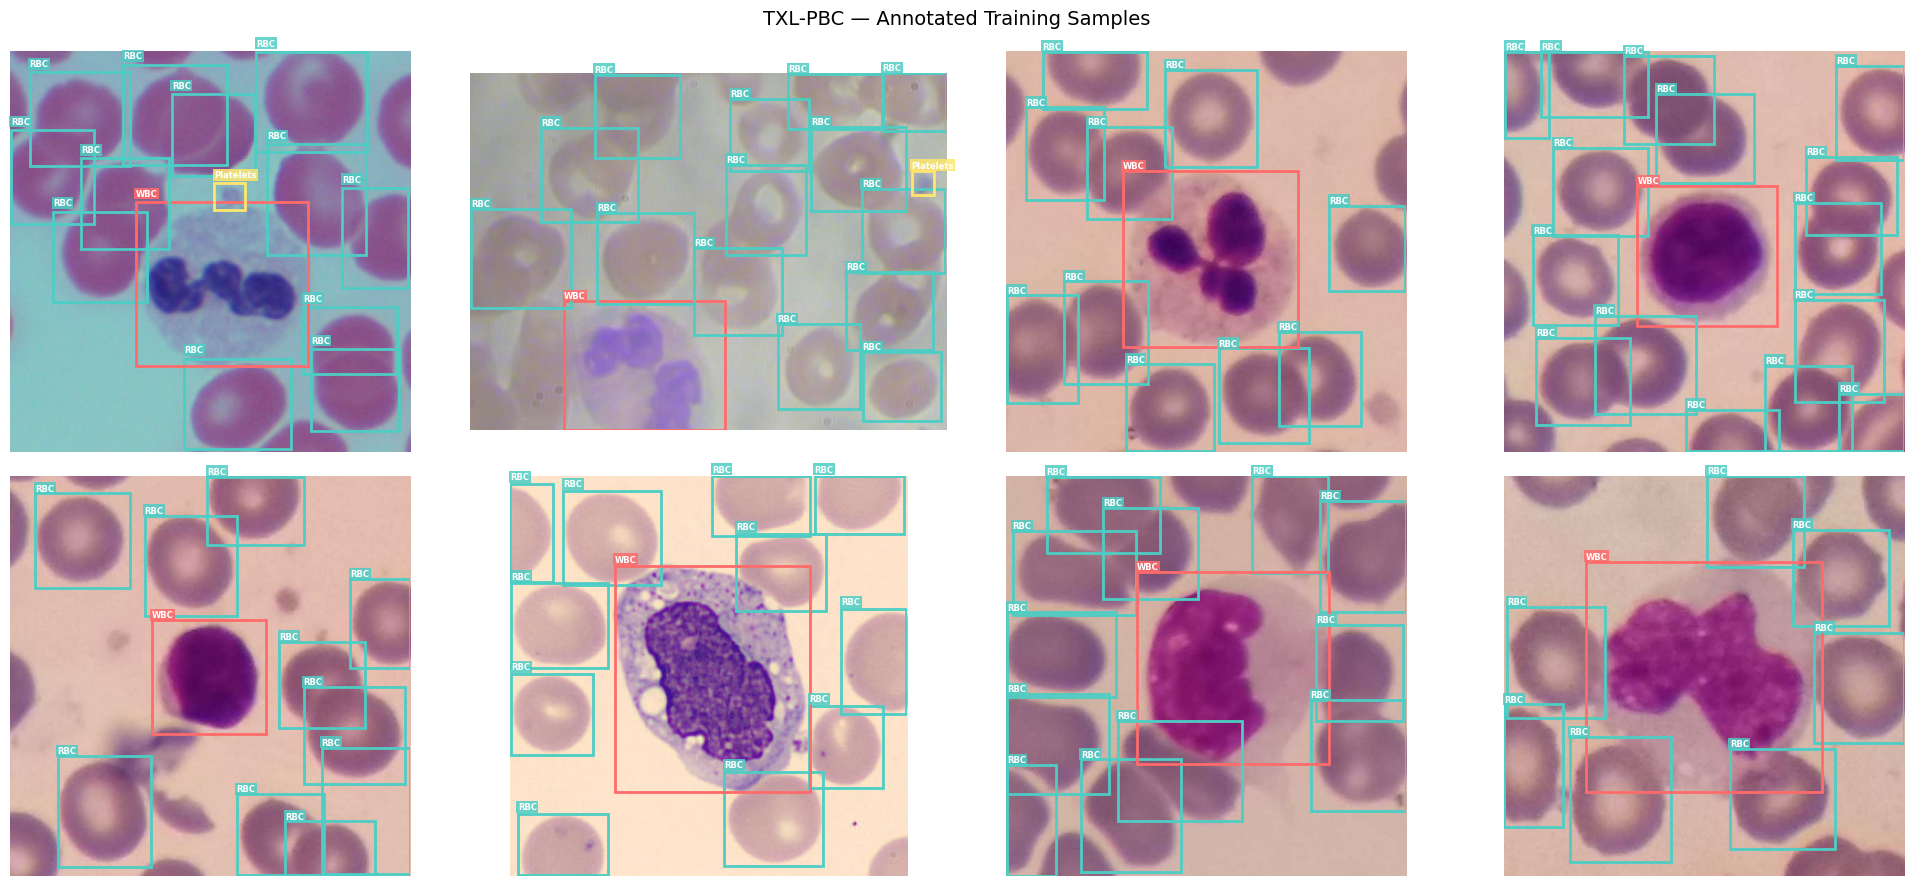
\includegraphics[width=0.95\textwidth]{figures/stage1_embedded_annotated_training_samples.png}
\caption{Annotated training images.}
\end{subfigure}\\[6pt]
\begin{subfigure}[t]{\textwidth}\centering
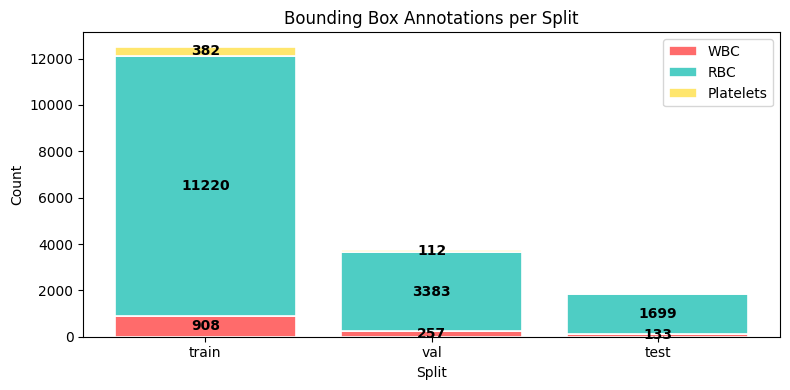
\includegraphics[width=0.62\textwidth]{figures/stage1_embedded_class_distribution_per_split.png}
\caption{Box annotations per split.}
\end{subfigure}
\caption{The TXL-PBC detection dataset: (a) example training images with their WBC, RBC and platelet boxes; (b) number of annotated boxes per class and split, counted from the raw label files (before Ultralytics removed a small number of duplicate labels). Red cells dominate every split.}
\label{fig:txl}
\end{figure}

\subsection{White-cell classification data: PBC}

The PBC dataset of Acevedo \emph{et al.} \cite{acevedo2020} contains 17{,}092 single-cell images of $360 \times 363$ pixels, recorded with a CellaVision DM96 analyser at the Hospital Clínic of Barcelona from individuals without infection, hematological disease or pharmacological treatment. Each image was labelled by clinical pathologists into one of eight classes: \emph{basophil, eosinophil, erythroblast, immature granulocyte (IG), lymphocyte, monocyte, neutrophil} and \emph{platelet}. The classes are moderately imbalanced (about 3{,}300 neutrophils and 1{,}200 basophils). The images were resized to $224 \times 224$ pixels. The final classifier (v2, Section~\ref{sec:method}) uses a class-stratified split into 11{,}963 training, 1{,}710 validation and 3{,}419 test images (70/10/20, seed 42); an earlier run (v1) used an unstratified 80/20 train/test split. Both splits are at image level, not grouped by donor, because the dataset does not identify the donor of each image.

\clearpage

\section{System Architecture and Design}\label{sec:arch}

\subsection{Architectural overview}

The lab assistant consists of two parts (Figure~\ref{fig:arch}). Two \emph{image-analysis stages} turn a smear image into structured findings: a detector that finds and counts the cells, and a classifier that assigns a type, an uncertainty level and a saliency map to every white cell. The \emph{domain expert} then interprets these findings using hematology knowledge. The expert can be run with a hosted model (GPT-4o inside a tool-using agent) or with the open, fine-tuned Llama model, and it can also be used on its own as a hematology question-answering system.

The pipeline is strictly feed-forward: every stage has a typed input and output, and each stage consumes only the structured output of the previous one, never the raw upstream data. This keeps each stage replaceable --- for example, the detector can be exchanged without retraining the classifier, and the language model can be exchanged without touching the vision stages --- and it produces an inspectable artefact at every step: a box overlay, a label with an uncertainty level, a heatmap, retrieved passages and a tool trace.

\begin{figure}[H]
\centering
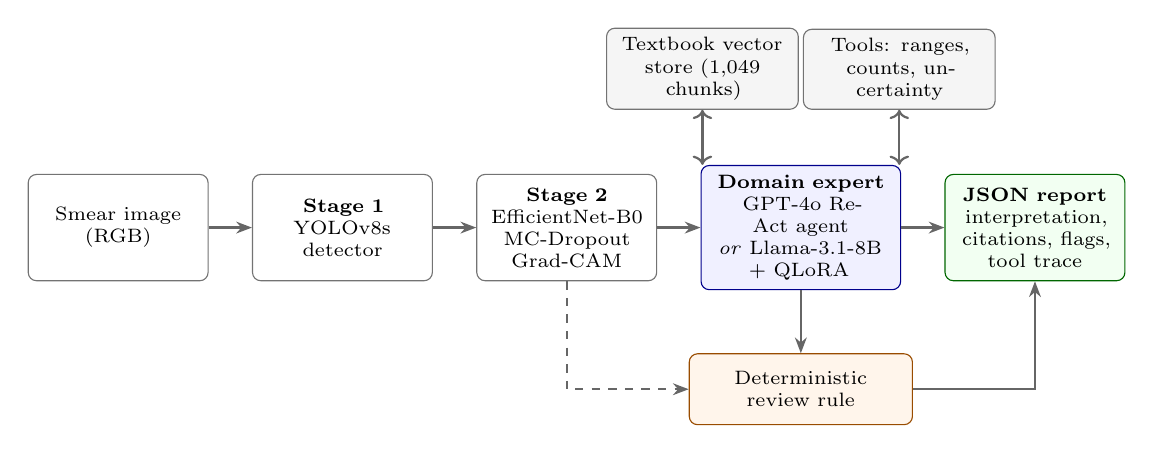
\begin{tikzpicture}[
  node distance=0.55cm,
  box/.style={draw=black!55, rounded corners=3pt, align=center, font=\scriptsize, minimum height=1.35cm, text width=2.05cm, fill=white},
  exp/.style={box, fill=blue!6, draw=blue!55!black, text width=2.3cm},
  kb/.style={box, fill=black!4, minimum height=0.8cm, text width=2.2cm},
  arr/.style={-{Stealth[length=2mm]}, thick, draw=black!60}]
\node[box] (img) {Smear image\\(RGB)};
\node[box, right=of img] (s1) {\textbf{Stage 1}\\YOLOv8s\\detector};
\node[box, right=of s1] (s2) {\textbf{Stage 2}\\EfficientNet-B0\\MC-Dropout\\Grad-CAM};
\node[exp, right=of s2] (de) {\textbf{Domain expert}\\GPT-4o ReAct agent\\\emph{or} Llama-3.1-8B\\+ QLoRA};
\node[box, right=of de, fill=green!5, draw=green!40!black] (rep) {\textbf{JSON report}\\interpretation,\\citations, flags,\\tool trace};
\node[kb, above=0.7cm of de, xshift=-1.25cm] (kb) {Textbook vector\\store (1{,}049 chunks)};
\node[kb, above=0.7cm of de, xshift=1.25cm] (tools) {Tools: ranges,\\counts, uncertainty};
\node[box, below=0.8cm of de, fill=orange!8, draw=orange!60!black, minimum height=0.9cm, text width=2.6cm] (rule) {Deterministic\\review rule};
\draw[arr] (img) -- (s1);
\draw[arr] (s1) -- (s2);
\draw[arr] (s2) -- (de);
\draw[arr] (de) -- (rep);
\draw[arr, <->] (kb.south) -- (kb.south |- de.north);
\draw[arr, <->] (tools.south) -- (tools.south |- de.north);
\draw[arr] (de.south) -- (rule.north);
\draw[arr, dashed] (s2.south) |- (rule.west);
\draw[arr] (rule.east) -| (rep.south);
\end{tikzpicture}
\caption{Architecture of the system. Stage~1 returns boxes, classes and confidences; Stage~2 returns, for every white cell, a label, confidence, entropy, uncertainty level and heatmap. The expert queries the knowledge base and tools and writes the report. The dashed arrow shows that the review rule reads the Stage-2 uncertainty directly, independently of the language model.}
\label{fig:arch}
\end{figure}

All runtime parameters --- model paths, thresholds, the number of MC-Dropout passes, chunk size, embedding model, number of retrieved chunks, language model, temperature and agent budget --- are set in a single \code{config.yaml} file. All inference goes through one orchestrator class, \code{BloodSmearPipeline}; the command-line interface and the web backend are thin wrappers around it.

\subsection{Stage 1: cell detection with YOLOv8}\label{sec:stage1}

Given an image $I$, Stage~1 returns a set of boxes $\mathcal{B}(I) = \{(x_1, y_1, x_2, y_2, c, p)_i\}$, where $c \in \{\text{WBC}, \text{RBC}, \text{Platelet}\}$ and $p$ is the detector's confidence. Boxes with $p < 0.50$ are discarded.

The detector is YOLOv8s \cite{jocher2023yolov8}, the ``small'' variant (about 11 million parameters) of a single-stage, anchor-free object detector. It consists of a convolutional backbone, a feature-pyramid neck that fuses information from several scales, and a decoupled head that predicts class scores and box coordinates. The small variant was chosen as a compromise between accuracy and speed on an ordinary laptop CPU. At inference the checkpoint is loaded once and kept in memory, and class names are normalised (\emph{Platelets} and \emph{Platelet} are unified, because source datasets use both). The white-cell boxes are cropped from the image and passed to Stage~2, and the per-class counts are passed to the domain expert.

\subsection{Stage 2: white-cell classification with uncertainty and saliency}\label{sec:stage2}

For each WBC crop, Stage~2 returns
\begin{equation}
  y(\text{crop}) = \big(\hat{c},\ \bar{p}_{(1)},\ H,\ v,\ b,\ \text{Grad-CAM}\big),
\end{equation}
the predicted class, its mean probability (confidence), the predictive entropy, the mean variance across passes, an uncertainty level $b \in \{\text{LOW}, \text{MEDIUM}, \text{HIGH}\}$, and a saliency overlay.

\paragraph{Classifier.} The backbone is EfficientNet-B0 \cite{tan2019efficientnet} from the \code{timm} library, pre-trained on ImageNet. Its 1{,}000-class head is replaced by a small multilayer head: Linear(1280$\to$1024) -- ReLU -- Dropout(0.3) -- Linear(1024$\to$512) -- ReLU -- Dropout(0.3) -- Linear(512$\to$8). The two dropout layers are what makes MC-Dropout possible.

\paragraph{Monte Carlo Dropout.} At prediction time the network is put into evaluation mode and then only its \code{nn.Dropout} modules are switched back to training mode; batch-normalisation layers stay in evaluation mode so that their statistics do not drift. Each crop is passed through the network $T = 20$ times, giving a $T \times C$ matrix of class probabilities. The mean $\bar{p}$ over the passes is the prediction, $\bar{p}_{(1)}$ is its largest entry, $H = -\sum_c \bar{p}_c \log \bar{p}_c$ is the predictive entropy, and $v$ is the per-class variance across passes averaged over the classes. The uncertainty level is then
\begin{equation}
b = \begin{cases}
\text{LOW} & \text{if } \bar{p}_{(1)} \ge 0.85 \text{ and } H < 0.3,\\
\text{MEDIUM} & \text{else if } \bar{p}_{(1)} \ge 0.65 \text{ and } H < 0.6,\\
\text{HIGH} & \text{otherwise.}
\end{cases}
\end{equation}
A HIGH cell is marked as \emph{flagged}. The thresholds are set in the configuration file; they were chosen by hand and have not been calibrated against error rates.

\paragraph{Grad-CAM.} For each crop, the predicted class score is back-propagated to the network's final convolutional layer (\code{conv\_head}), the Grad-CAM map (Equation~2) is up-sampled to $224 \times 224$ and blended over the crop with an opacity of 0.45. The resulting image is returned with the prediction and shown in the user interface.

\subsection{Stage 3: domain-expert reasoning --- knowledge base and retrieval (RAG)}\label{sec:kb}

The 1{,}049 textbook chunks (Section~\ref{sec:corpus}) are embedded with the sentence-transformer \code{all-MiniLM-L6-v2} \cite{reimers2019,wang2020minilm}, a six-layer model that maps a text to a 384-dimensional vector and runs quickly on a CPU. The vectors are stored in a persistent ChromaDB collection \cite{chroma} with cosine distance, so the index is built once and re-used; it is rebuilt automatically if the number of stored chunks does not match the corpus. For a query, the query text is embedded with the same model and the five most similar chunks are returned with their source and chunk index. The complete pipeline is shown in Figure~\ref{fig:rag}. An optional web-search extension, restricted to an allow-list of medical domains (e.g.\ NCBI, MedlinePlus, WHO), exists but is disabled in all experiments for reproducibility.

\begin{figure}[H]
\centering
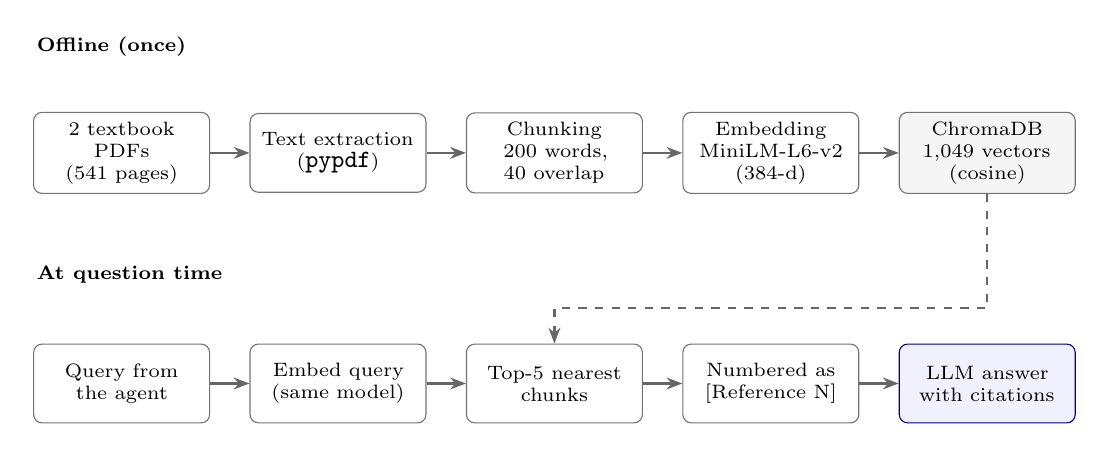
\begin{tikzpicture}[
  node distance=0.5cm,
  st/.style={draw=black!55, rounded corners=3pt, align=center, font=\scriptsize, minimum height=1.0cm, text width=2.0cm, fill=white},
  db/.style={st, fill=black!4},
  arr/.style={-{Stealth[length=2mm]}, thick, draw=black!60}]
% offline row
\node[font=\scriptsize\bfseries, anchor=west] (off) at (-1.2,1.35) {Offline (once)};
\node[st] (pdf) at (0,0) {2 textbook PDFs\\(541 pages)};
\node[st, right=of pdf] (ext) {Text extraction\\(\code{pypdf})};
\node[st, right=of ext] (chk) {Chunking\\200 words,\\40 overlap};
\node[st, right=of chk] (emb) {Embedding\\MiniLM-L6-v2\\(384-d)};
\node[db, right=of emb] (vdb) {ChromaDB\\1{,}049 vectors\\(cosine)};
% online row
\node[font=\scriptsize\bfseries, anchor=west] (on) at (-1.2,-1.55) {At question time};
\node[st, below=1.9cm of pdf] (q) {Query from\\the agent};
\node[st, right=of q] (qe) {Embed query\\(same model)};
\node[st, right=of qe] (top) {Top-5 nearest\\chunks};
\node[st, right=of top] (ref) {Numbered as\\{[}Reference N{]}};
\node[st, right=of ref, fill=blue!6, draw=blue!55!black] (llm) {LLM answer\\with citations};
\draw[arr] (pdf) -- (ext); \draw[arr] (ext) -- (chk); \draw[arr] (chk) -- (emb); \draw[arr] (emb) -- (vdb);
\draw[arr] (q) -- (qe); \draw[arr] (qe) -- (top); \draw[arr] (top) -- (ref); \draw[arr] (ref) -- (llm);
\draw[arr, dashed] (vdb.south) |- ($(top.north)+(0,0.45)$) -- (top.north);
\end{tikzpicture}
\caption{The retrieval-augmented generation (RAG) pipeline. The knowledge base is built once; at question time the agent's query is embedded with the same model and the five most similar chunks are returned, numbered so that the model can cite them.}
\label{fig:rag}
\end{figure}

\subsection{Stage 3, backend A: GPT-4o with tools (ReAct agent)}\label{sec:agent}

The main runtime expert is GPT-4o \cite{openai2024gpt4o}, called at temperature 0.1 through the OpenAI API. GPT-4o was chosen because it follows structured-output and tool-calling instructions reliably and needs no local GPU. The model is wrapped in a LangGraph ReAct agent \cite{yao2023react,langgraph} with the five tools listed in Table~\ref{tab:tools}.

\begin{table}[H]
\centering
\caption{Tools available to the domain-expert agent.}
\label{tab:tools}
\small
\begin{tabularx}{\textwidth}{>{\raggedright\arraybackslash}p{5.6cm} X}
\toprule
\textbf{Tool} & \textbf{Purpose} \\
\midrule
\code{query\_knowledge\_base} & Takes a search query; retrieves the top-5 textbook chunks and numbers them as \code{[Reference N]}. \\
\code{lookup\_lab\_reference\_ranges} & Takes a parameter name; returns a typical adult reference range (e.g.\ monocytes 2--8\,\% of WBC). \\
\code{interpret\_differential} & Takes the differential as JSON; compares each class percentage with its reference range and reports LOW/HIGH/normal. \\
\code{get\_uncertainty\_summary} & Returns the Stage-2 MC-Dropout statistics (number of flagged cells). \\
\code{get\_detection\_counts} & Returns the Stage-1 cell counts for the field of view. \\
\bottomrule
\end{tabularx}
\end{table}

The system prompt tells the agent to call the knowledge base one to three times to ground its claims, to look up reference ranges before calling a value abnormal, to review the uncertainty summary before making confident statements, to cite evidence as \code{[Reference N]}, to give differential rather than definitive diagnoses, and to remember that the counts are per microscope field and must not be converted into clinical concentrations. The final message must be a JSON object with the fields \code{clinical\_interpretation}, \code{key\_findings}, \code{differential\_diagnoses}, \code{recommendations}, \code{safety\_flags}, \code{requires\_expert\_review} and \code{confidence\_assessment}. The number of reasoning steps is bounded through LangGraph's recursion limit (derived from a configured maximum of six iterations), and every tool call and tool result is returned to the user as the \emph{agent trace}.

A simpler \emph{linear} mode is also available: one retrieval followed by one LLM call with the retrieved chunks in the prompt. In linear mode the code checks that the cited reference numbers actually exist among the retrieved chunks, and it adds an \code{INSUFFICIENT\_EVIDENCE} flag if no valid citation or no differential diagnosis is returned.

The language-model client talks to any OpenAI-compatible endpoint. Replacing GPT-4o by a self-hosted model therefore only requires changing the model name in \code{config.yaml} and the \code{OPENAI\_BASE\_URL} environment variable.

\subsection{Stage 3, backend B: a fine-tuned open-weight model}\label{sec:ft}

The second form of the expert is an open-weight model adapted to the domain, which can run on local hardware. The base model is \textbf{Llama-3.1-8B-Instruct} \cite{grattafiori2024llama3}, loaded in 4-bit precision, and it is adapted with \textbf{QLoRA} \cite{dettmers2023qlora}: LoRA adapters of rank $r=16$ ($\alpha = 32$, no dropout) are attached to all attention and feed-forward projections (\code{q, k, v, o, gate, up, down}), which adds 41.9 million trainable parameters --- 0.52\,\% of the model's 8.07 billion. The adapter is trained on the 1{,}890 training pairs (Section~\ref{sec:qa-data}), so the model learns to answer hematology questions in the form of the textbook-grounded answers. The resulting adapter (about 42 million parameters, roughly 84\,MB in 16-bit precision) can be served, for example with vLLM, behind an OpenAI-compatible endpoint and selected in the configuration without changing any other part of the system. Training details are given in Section~\ref{sec:ft-train}.

It is important to note what the training examples contain: a system prompt, a question and an answer --- but \emph{not} the textbook passage. The fine-tuned model therefore learns to answer from its weights, not to read and cite a retrieved passage. This design choice turns out to matter for how its citations should be interpreted (Section~\ref{sec:res-de}).

\subsection{Safety logic: the expert-review rule}\label{sec:safety}

Two design principles guide the safety behaviour. First, safety-relevant information is always passed forward and shown: every detection carries its confidence, every classified cell its uncertainty level and heatmap, every interpretation its tool trace. Second, the decision whether a human must review the case is not left to the language model alone. The flag \code{requires\_expert\_review} starts from the model's own judgement, but deterministic code \emph{forces it to true} whenever at least one Stage-2 cell is flagged as HIGH uncertainty, and adds a \code{HIGH\_UNCERTAINTY} safety flag. In linear mode, missing citations also force the flag. A second rule, added after the case study in Section~\ref{sec:case} revealed the gap, checks the \emph{number} of classified white cells: if it is below a configurable minimum (\code{llm.safety.min\_wbc\_for\_differential}, default 100, following the convention of counting at least 100 cells for a differential \cite{clsi2007h20}), an \code{INSUFFICIENT\_CELL\_COUNT} flag is added and review is forced. Both reasoners are also told the cell count and instructed not to interpret percentages when it is insufficient. The rules are implemented in \code{src/utils/safety\_rules.py} and applied by the pipeline after either reasoner has answered, so they hold in both modes. The code can only raise the flag, never lower it. Stage-1 detection confidence does not influence the flag.

\subsection{Software implementation and user interface}\label{sec:software}

The system is implemented as a Python library (\code{src/}) with a FastAPI backend (\code{backend/}) and a React + TypeScript web interface (\code{frontend/}). The backend exposes \code{GET /api/health}, \code{GET /api/samples} and \code{POST /api/analyze}; the latter accepts an image (and optionally a JSON object with CBC laboratory values) and returns the full JSON result. The pipeline is loaded lazily on the first request. The interface shows five panels: the detection overlay with cell counts, the WBC differential with per-cell uncertainty, the Grad-CAM heatmaps, the expert's interpretation with citations and safety flags, and the agent trace (Figures~\ref{fig:ui-a} and~\ref{fig:ui-b}). Thirty-four automated \code{pytest} tests cover configuration loading, batch logic, parsing of model output, retrieval fall-backs, the uncertainty schema, the CBC analyser, the minimum-cell rule and the prompts given to the reasoners. The 29 tests that do not require PyTorch and the trained model files were run for this thesis and all passed; the remaining five load the models and must be run in the project's full environment. The training notebooks for all three models are included and can be run on Google Colab.

The optional CBC input deserves a remark. A small module converts laboratory values (WBC, hemoglobin, MCV, platelets, etc.) into findings such as \emph{leukocytosis} or \emph{microcytosis} with a mild/moderate/severe grade. The findings are added to the prompt of both reasoners (in the agent's input message, and in linear mode also to the retrieval query), together with an instruction to reconcile them with the image findings. The web interface does not yet have a CBC input field, so CBC values can currently only be supplied through the API. Because no experiment in this thesis uses CBC values, this feature is presented as an implemented extension, not as an evaluated result.

\begin{figure}[H]
\centering
\begin{subfigure}{\textwidth}\centering
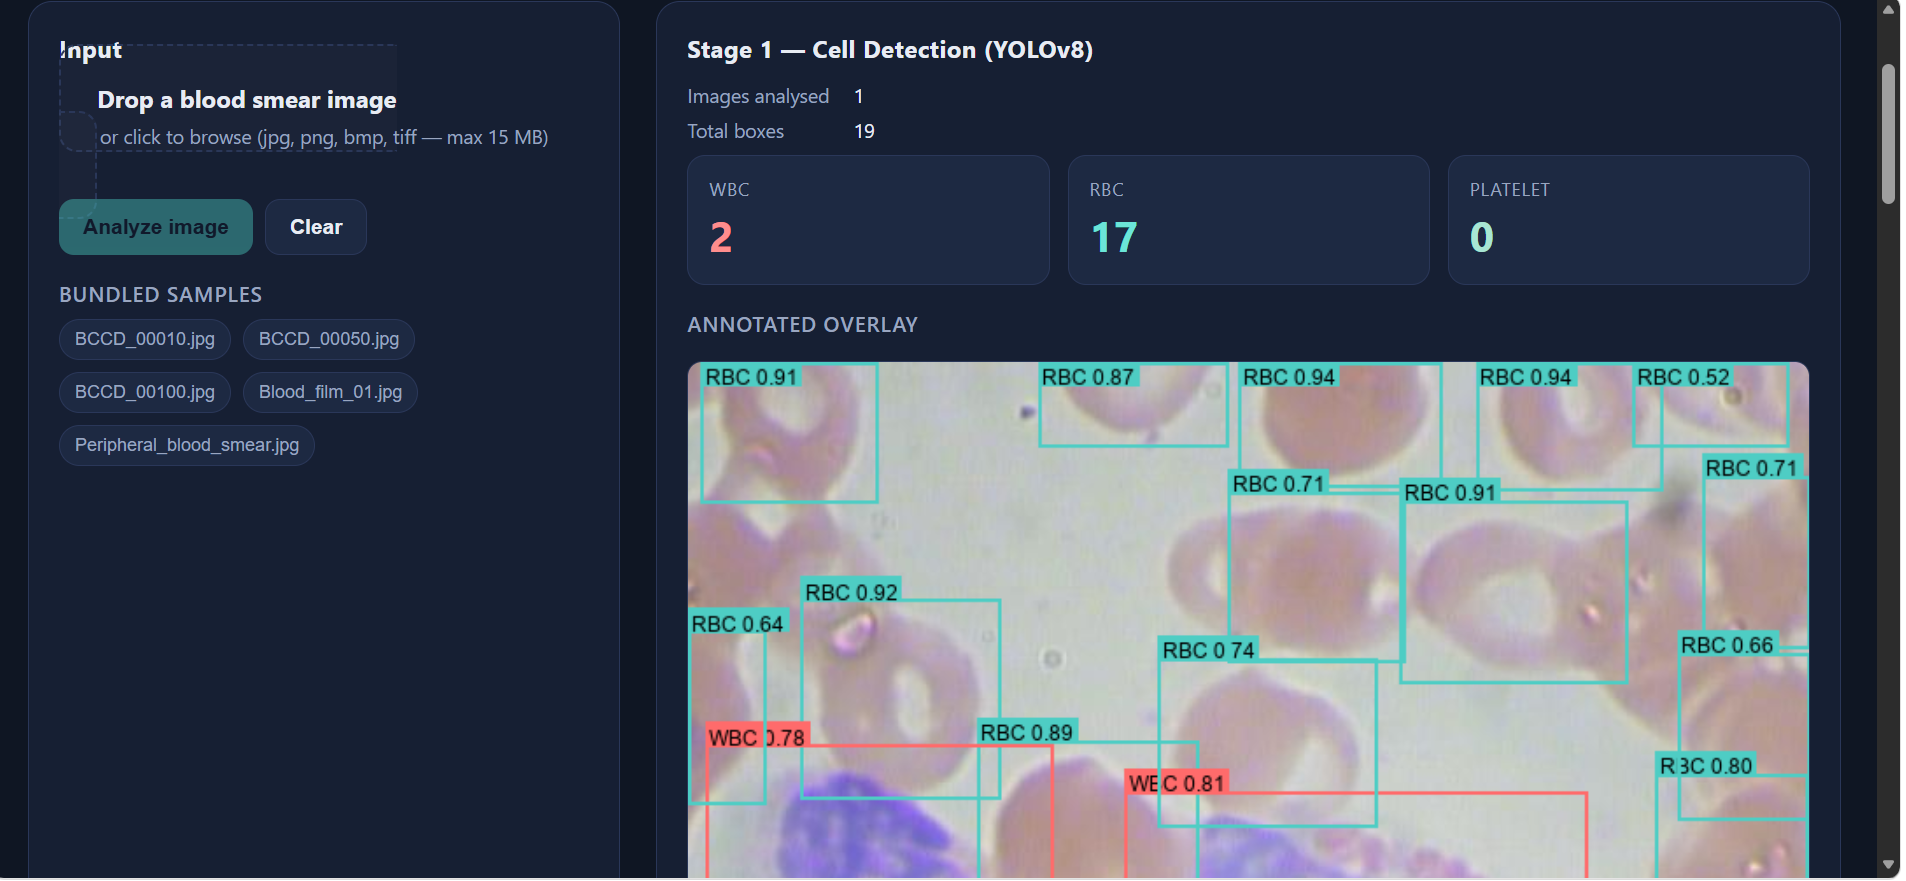
\includegraphics[width=0.95\textwidth]{figures/01_detection.png}
\caption{Detection panel: boxes and per-class counts.}
\end{subfigure}\\[6pt]
\begin{subfigure}{\textwidth}\centering
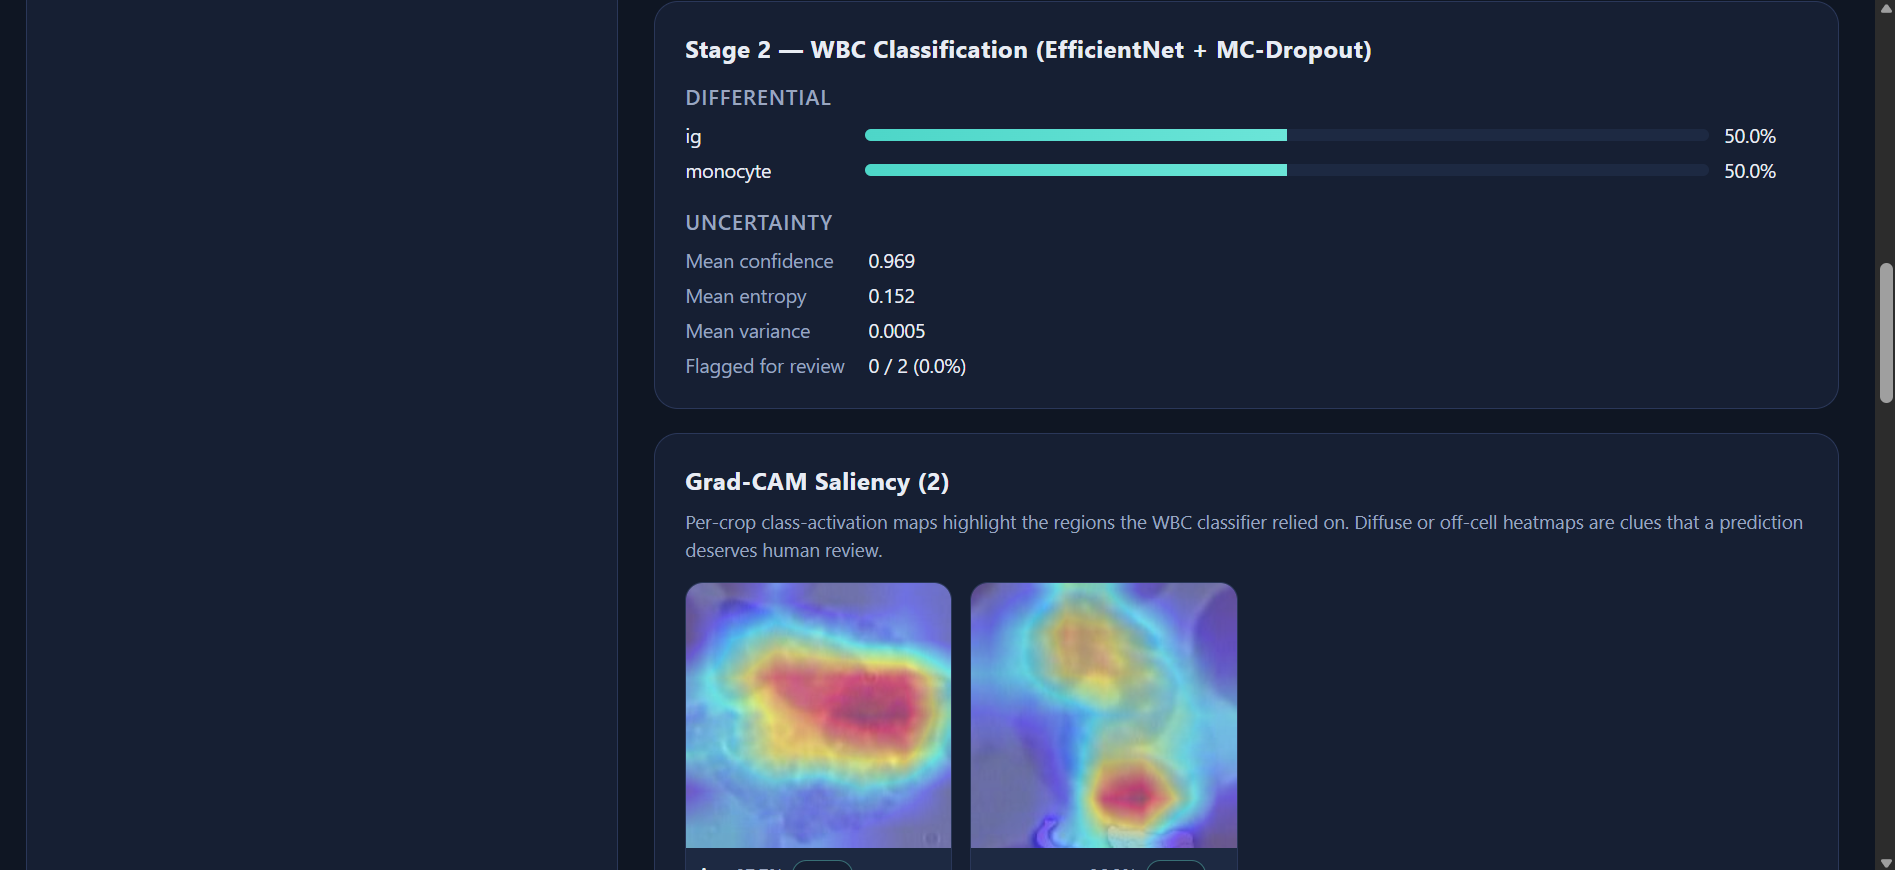
\includegraphics[width=0.95\textwidth]{figures/02_classification_gradcam.png}
\caption{WBC differential, per-cell uncertainty and Grad-CAM heatmaps.}
\end{subfigure}
\caption{Web interface: image-analysis stages, on sample image BCCD\_00100.}
\label{fig:ui-a}
\end{figure}

\begin{figure}[H]
\centering
\begin{subfigure}{\textwidth}\centering
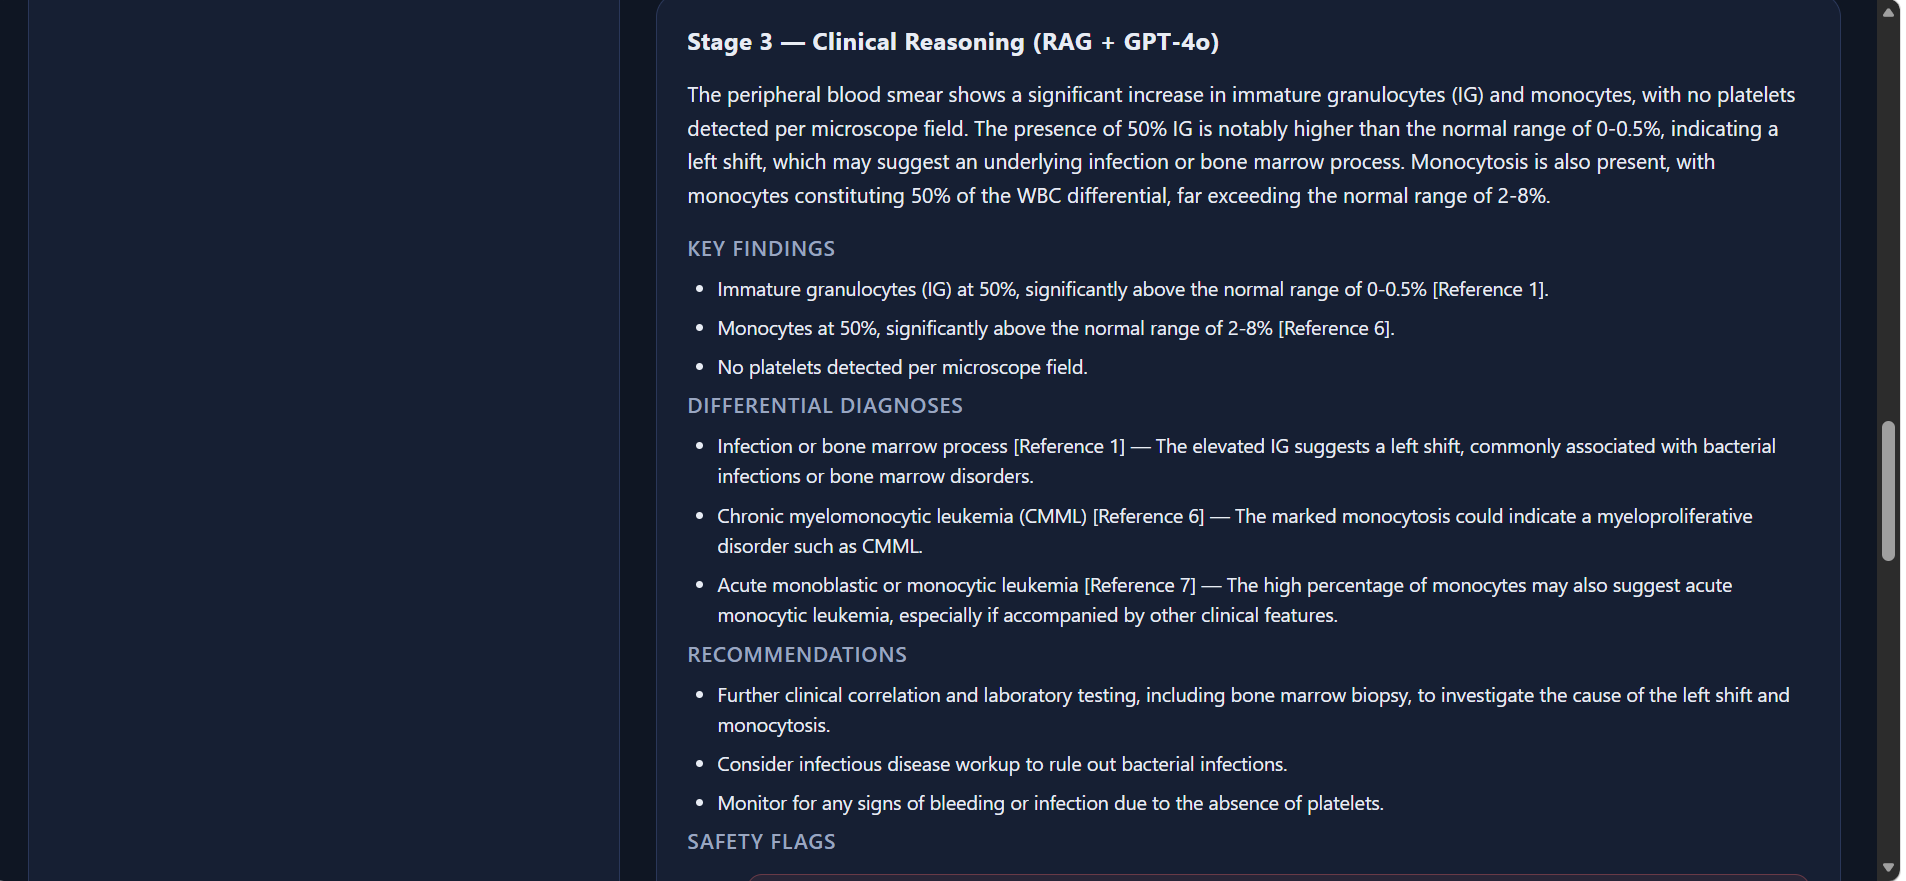
\includegraphics[width=0.95\textwidth]{figures/03_reasoning.png}
\caption{The expert's interpretation with citations and safety flags.}
\end{subfigure}\\[6pt]
\begin{subfigure}{\textwidth}\centering
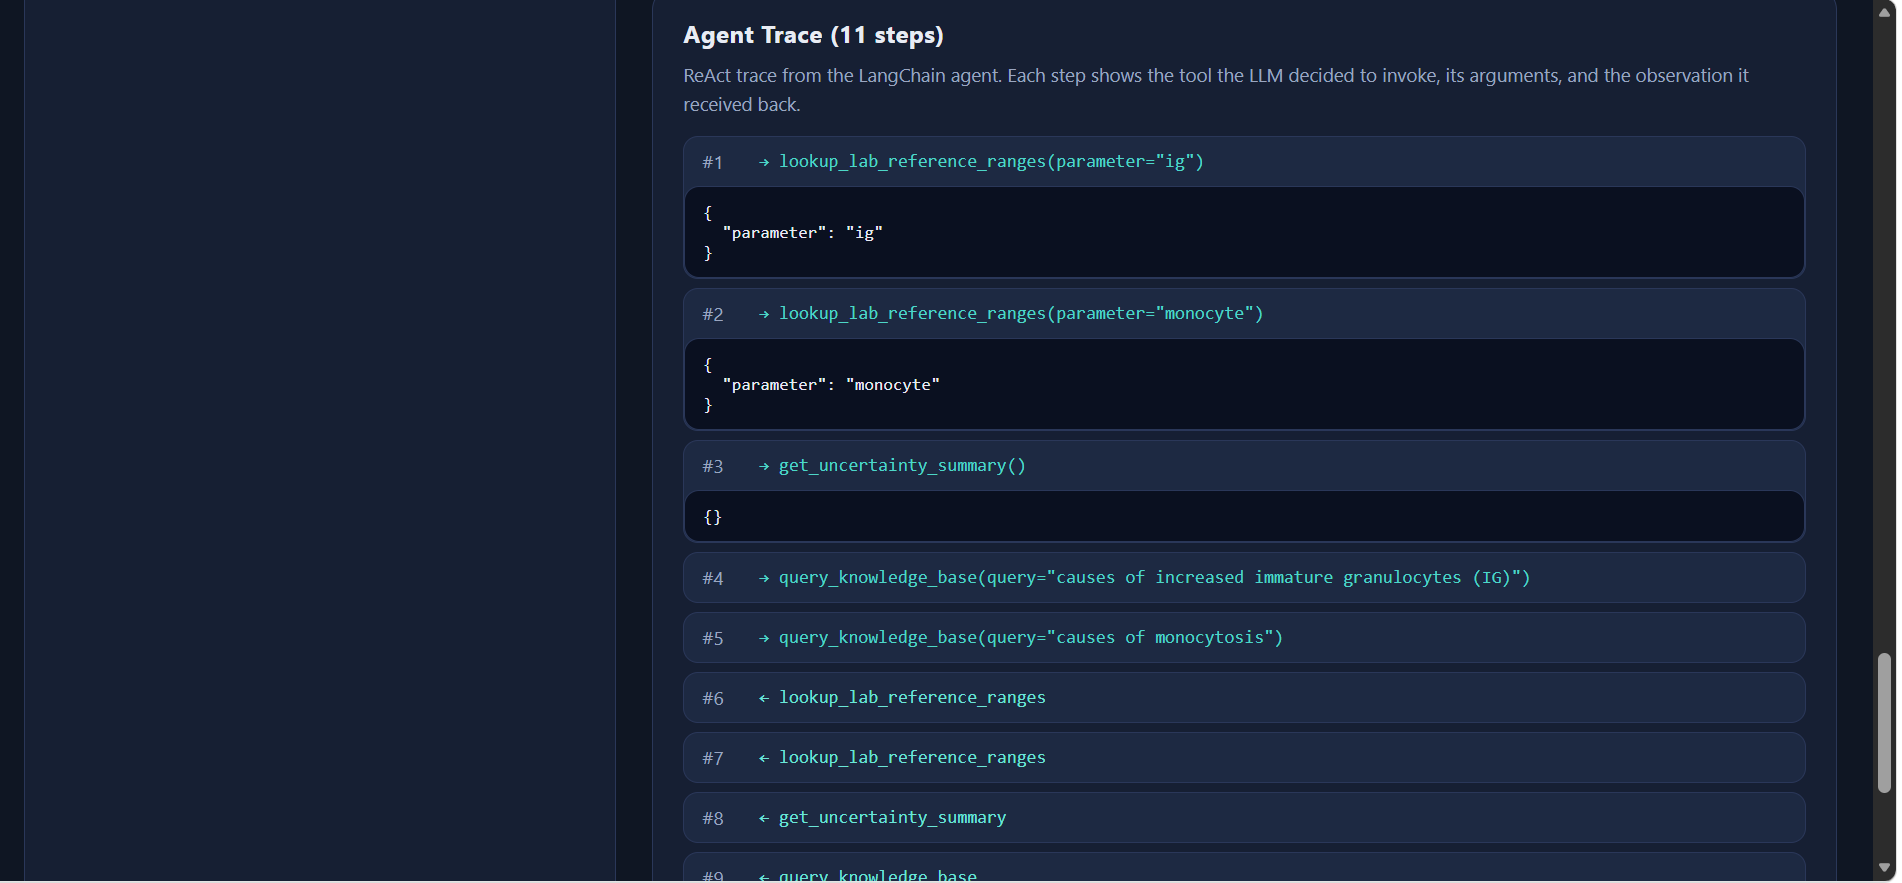
\includegraphics[width=0.95\textwidth]{figures/04_agent_trace.png}
\caption{Agent trace: the sequence of tool calls and results.}
\end{subfigure}
\caption{Web interface: domain-expert output.}
\label{fig:ui-b}
\end{figure}

\clearpage

\section{Research Methodology}\label{sec:method}

This chapter describes how the three models were trained and how the image-analysis stages and the domain expert were evaluated. All training was done on Google Colab with a single NVIDIA T4 GPU (16\,GB).

\subsection{Training the image-analysis models}

\paragraph{YOLOv8s.} The detector was fine-tuned from the COCO-pre-trained \code{yolov8s.pt} checkpoint for 50 epochs (0.30 hours on the T4) with the settings in Table~\ref{tab:yolo}. All flips and rotations are physically plausible for a smear, which has no preferred orientation.

\begin{table}[H]
\centering
\caption{YOLOv8s training settings (from the Ultralytics training log).}
\label{tab:yolo}
\small
\begin{tabular}{ll@{\hspace{1.5cm}}ll}
\toprule
\textbf{Setting} & \textbf{Value} & \textbf{Setting} & \textbf{Value} \\
\midrule
Epochs & 50 & Image size & $640 \times 640$ \\
Batch size & 8 & Optimiser & AdamW \\
Initial LR & 0.001 & Final LR factor & 0.01 (linear) \\
Momentum & 0.937 & Weight decay & $5 \times 10^{-4}$ \\
Warm-up epochs & 3 & Mosaic & 1.0 (off in last 10 epochs) \\
HSV jitter (h/s/v) & 0.015 / 0.7 / 0.4 & Rotation & $\pm 10^\circ$ \\
Flip (horizontal/vertical) & 0.5 / 0.5 & Seed & 0 (deterministic) \\
\bottomrule
\end{tabular}
\end{table}

\paragraph{EfficientNet-B0.} The classifier was trained in two phases (the same recipe was used in both training runs described below). In Phase~1 the backbone was frozen and only the new head was trained (40 epochs at most, batch size 32, Adam with learning rate $10^{-3}$, learning rate halved when accuracy stopped improving for three epochs, early stopping with patience five). In Phase~2 all layers were unfrozen and trained for 10 epochs with a ten times smaller learning rate ($10^{-4}$). The augmentations were random horizontal (p = 0.5) and vertical (p = 0.3) flips, random affine transforms ($\pm 25^\circ$, scale 0.8--1.2) and colour jitter.

\noindent\fbox{\parbox{\dimexpr\textwidth-2\fboxsep-2\fboxrule}{\small
\textbf{Two training runs.} The \emph{original run (v1)} used an 80/20 train/test split and had no separate validation set: the accuracy monitored after every epoch, the learning-rate scheduler and the choice of the saved checkpoint were all based on the \emph{test} images, so its test accuracy is optimistic. This flaw was found during the preparation of the thesis, and the classifier was therefore retrained in a \emph{corrected run (v2)} with the same architecture and recipe but a proper protocol: a class-stratified 70/10/20 split into 11{,}963 training, 1{,}710 validation and 3{,}419 test images (sorted file lists, seed 42), the learning-rate schedule, early stopping and checkpoint choice based on the validation set only, and a single evaluation on the test set. One non-image file (a macOS \code{.DS\_} metadata file with a \code{.jpg} extension) was skipped. All classification results reported in Chapter~\ref{sec:results} are from v2 unless stated otherwise; the v2 checkpoint is also the one configured in the system.}}

\subsection{Evaluation of the image-analysis stages}

\paragraph{Detection.} The YOLOv8s model was evaluated once on the 126-image TXL-PBC test split with the standard object-detection metrics: precision, recall, mean average precision at an intersection-over-union threshold of 0.50 (mAP@0.50), and mAP averaged over thresholds 0.50--0.95. The checkpoint was selected on the validation split.

\paragraph{Classification.} The EfficientNet-B0 model (v2) was evaluated once on its 3{,}419 test images with top-1 accuracy, per-class precision, recall and F1, and a normalised confusion matrix.

\paragraph{Uncertainty.} The test images were also passed through the classifier with MC-Dropout ($T = 20$, exactly as in the running system) to measure three things: (i) \emph{calibration}, as the expected calibration error (ECE, 15 equal-width confidence bins) and a reliability diagram, for both the MC-Dropout mean and a single deterministic pass; (ii) how well the uncertainty scores \emph{detect errors}, as the area under the ROC curve (AUROC) of $1-\bar{p}_{(1)}$, entropy and variance for separating misclassified from correctly classified cells; and (iii) the accuracy of the cells in each uncertainty level (LOW, MEDIUM, HIGH) with the thresholds of the configuration file.

\subsection{Training the domain-expert model}\label{sec:ft-train}

The Llama model was fine-tuned with the Unsloth library \cite{unsloth} (version 2026.9.12, with Transformers 5.5.0 and PyTorch 2.11) and the supervised fine-tuning trainer of the TRL library, using the settings in Table~\ref{tab:qlora}. Each training example was rendered with the Llama-3.1 chat template and the loss was computed on the full sequence. Training took 474 optimisation steps and 49.8 minutes. The loss fell from 2.67 at the first logged step to about 0.57 at the end of the first epoch and 0.42 at the end of the second (Figure~\ref{fig:loss}); the drop at the start of the second epoch is the typical sign that the model has begun to memorise the training answers, which is why training was limited to two epochs.

\begin{table}[H]
\centering
\caption{QLoRA fine-tuning settings.}
\label{tab:qlora}
\small
\begin{tabular}{ll}
\toprule
\textbf{Setting} & \textbf{Value} \\
\midrule
Base model & \code{unsloth/Meta-Llama-3.1-8B-Instruct-bnb-4bit} (4-bit) \\
LoRA rank / alpha / dropout & 16 / 32 / 0.0 \\
Target modules & \code{q, k, v, o, gate, up, down} projections \\
Trainable parameters & 41{,}943{,}040 (0.52\,\% of 8.07\,B) \\
Training examples & 1{,}890 \\
Epochs / steps & 2 / 474 \\
Batch size & 2 per device $\times$ 4 gradient accumulation = 8 \\
Learning rate & $2 \times 10^{-4}$, linear decay, 10 warm-up steps \\
Optimiser / weight decay & AdamW (8-bit) / 0.01 \\
Maximum sequence length & 2{,}048 tokens \\
Precision & FP16 (the T4 does not support BF16) \\
Seed & 42 \\
Training time & 49.8 min on one T4 \\
\bottomrule
\end{tabular}
\end{table}

\begin{figure}[H]
\centering
\includegraphics[width=0.78\textwidth]{figures/qlora_training_loss.pdf}
\caption{Training loss of the QLoRA fine-tuning, logged every 10 steps.}
\label{fig:loss}
\end{figure}

\begin{figure}[H]
\centering
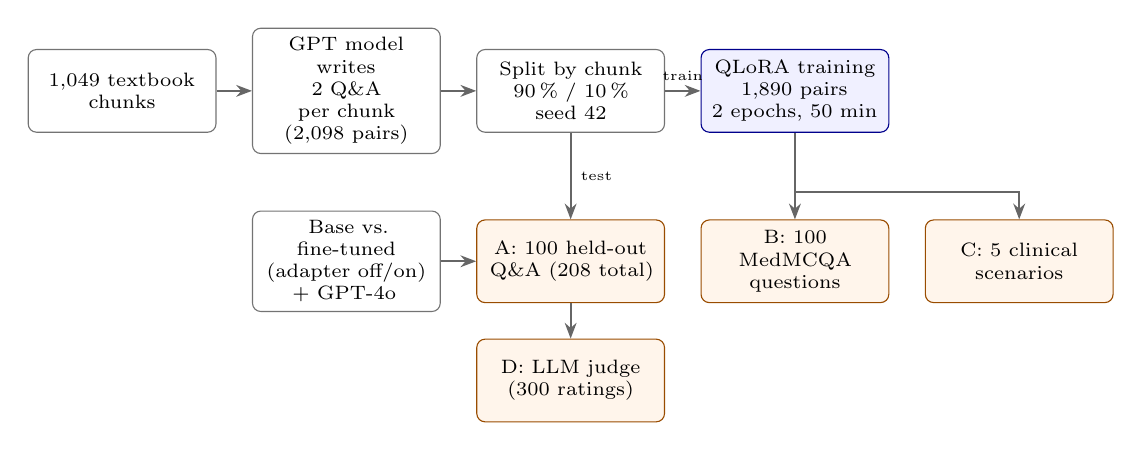
\begin{tikzpicture}[
  node distance=0.45cm and 0.45cm,
  st/.style={draw=black!55, rounded corners=3pt, align=center, font=\scriptsize, minimum height=1.05cm, text width=2.15cm, fill=white},
  ev/.style={st, fill=orange!8, draw=orange!60!black},
  arr/.style={-{Stealth[length=2mm]}, thick, draw=black!60}]
\node[st] (ch) {1{,}049 textbook\\chunks};
\node[st, right=of ch] (gen) {GPT model writes\\2 Q\&A per chunk\\(2{,}098 pairs)};
\node[st, right=of gen] (sp) {Split by chunk\\90\,\% / 10\,\%\\seed 42};
\node[st, right=of sp, fill=blue!6, draw=blue!55!black] (tr) {QLoRA training\\1{,}890 pairs\\2 epochs, 50 min};
\node[ev, below=1.1cm of sp] (a) {A: 100 held-out\\Q\&A (208 total)};
\node[ev, right=of a] (b) {B: 100 MedMCQA\\questions};
\node[ev, right=of b] (c) {C: 5 clinical\\scenarios};
\node[ev, below=0.45cm of a] (d) {D: LLM judge\\(300 ratings)};
\node[st, left=of a] (sys) {Base vs.\ fine-tuned\\(adapter off/on)\\+ GPT-4o};
\draw[arr] (ch) -- (gen); \draw[arr] (gen) -- (sp); \draw[arr] (sp) -- node[above,font=\tiny]{train} (tr);
\draw[arr] (sp) -- node[right,font=\tiny]{test} (a);
\draw[arr] (tr.south) |- ($(b.north)+(0,0.35)$) -- (b.north);
\draw[arr] ($(b.north)+(0,0.35)$) -| (c.north);
\draw[arr] (sys) -- (a);
\draw[arr] (a) -- (d);
\end{tikzpicture}
\caption{Workflow of the domain-expert experiment: data generation, chunk-level split, QLoRA training and the four evaluations.}
\label{fig:ftflow}
\end{figure}

\subsection{Evaluation protocol for the domain expert}\label{sec:eval}

The evaluation compares three systems: the original \textbf{Llama-3.1-8B-Instruct (base)}, the same model with the \textbf{QLoRA adapter (ours)}, and \textbf{GPT-4o} as a reference for a strong hosted model. The base and fine-tuned answers come from the \emph{same} loaded model with the adapter switched off and on, so any difference is caused by the adapter alone. All three systems received the same system prompt as used in training, the questions were asked \emph{without} retrieved passages (the test measures the model, not the retrieval), and decoding was deterministic (greedy decoding for Llama; temperature 0 for GPT-4o). Answers were limited to 256 new tokens for Llama and 300 for GPT-4o.

\paragraph{A. In-domain held-out questions.} The first 100 of the 208 held-out questions were answered by all three systems and compared with the reference answers using:
\begin{itemize}
  \item \textbf{ROUGE-L F1} \cite{lin2004rouge}: word-level overlap based on the longest common subsequence (with stemming);
  \item \textbf{semantic similarity}: the cosine similarity between the \code{all-MiniLM-L6-v2} embeddings of the answer and of the reference answer;
  \item \textbf{source marker rate}: the share of answers that contain a source marker (``Source:'', ``[Reference'', or a textbook file name). This measures the citation \emph{format}, not whether the citation is correct;
  \item \textbf{answer length} in words.
\end{itemize}

\paragraph{B. External multiple-choice questions.} The 100 MedMCQA questions were given to the base and fine-tuned models with the four options and the instruction to answer with a single letter; the first letter A--D in the answer was taken as the choice. Random guessing gives 25\,\%. GPT-4o was not evaluated on this set.

\paragraph{C. Qualitative comparison.} Five clinical questions written for this thesis --- including one that describes the two-cell differential of the case study --- were answered by the base and the fine-tuned model and inspected by hand. In addition, all in-domain answers were checked automatically for invented bibliographic references (a named book title, author or edition), since no source was ever given to the models.

\paragraph{Statistics.} Because all systems answer the same questions, differences were tested in a paired way: a 95\,\% bootstrap confidence interval (5{,}000 resamples of the 100 questions) for the difference in mean ROUGE-L, and an exact McNemar test for the difference in multiple-choice accuracy. These statistics were computed after the Colab run from the saved answers (\code{results/domain\_expert/evaluation\_report.json}).

\paragraph{D. LLM-as-judge.} Following \cite{zheng2023judge}, GPT-4o-mini (temperature 0) rated every in-domain answer of all three systems --- 300 ratings --- on two 1--5 scales: \emph{faithfulness} (agreement with the textbook reference answer, no unsupported or contradicting claims) and \emph{clinical correctness} (medical accuracy). The judge saw the question, the reference answer and one model answer at a time, never the name of the system, and was told that a source line earns no credit and that length does not matter. The judging step of the Colab notebook failed because of a string-formatting error, so the ratings were produced afterwards from the saved answers with a corrected stand-alone script (\code{scripts/judge\_domain\_expert.py}). Differences between systems are reported with paired bootstrap confidence intervals. An LLM judge is not a substitute for clinicians, and GPT-4o-mini may be biased towards the style of its larger sibling GPT-4o.

\clearpage

\section{Results and Discussion}\label{sec:results}

This chapter first presents the results of the two image-analysis stages and then the evaluation of the domain-expert LLM, which is the central question of the thesis topic. It continues with an end-to-end case study of a real run of the lab assistant, and ends with a discussion of the research questions and the limitations.

\subsection{Stage 1: detection results}

On the 126-image TXL-PBC test split, the detector reached a mAP@0.50 of 0.985 and a mAP@0.50:0.95 of 0.876 (Table~\ref{tab:det}). White cells were found with a recall of 1.000, so every annotated white cell in the test split reaches the classifier. Red cells have the lowest recall (0.943), as expected for densely packed, overlapping cells, and platelets --- the smallest and rarest objects (49 test instances) --- have the lowest precision and mAP. The normalised confusion matrix is nearly diagonal; the errors are missed cells and false detections against the background rather than confusions between classes (Figure~\ref{fig:det}). The training and validation losses decreased steadily over the 50 epochs and the validation metrics levelled off without a late decline, so there is no sign of over-fitting (Figure~\ref{fig:yolo-curves}).

\begin{table}[H]
\centering
\caption{YOLOv8s results on the TXL-PBC test split.}
\label{tab:det}
\small
\begin{tabular}{lrrcccc}
\toprule
\textbf{Class} & \textbf{Images} & \textbf{Instances} & \textbf{Precision} & \textbf{Recall} & \textbf{mAP@0.50} & \textbf{mAP@0.50:0.95} \\
\midrule
WBC & 126 & 131 & 0.992 & 1.000 & 0.995 & 0.889 \\
RBC & 126 & 1{,}688 & 0.977 & 0.943 & 0.990 & 0.906 \\
Platelet & 34 & 49 & 0.958 & 0.939 & 0.970 & 0.834 \\
\midrule
\textbf{All} & 126 & 1{,}868 & \textbf{0.976} & \textbf{0.961} & \textbf{0.985} & \textbf{0.876} \\
\bottomrule
\end{tabular}
\end{table}

\begin{figure}[H]
\centering
\begin{subfigure}[t]{0.62\textwidth}\centering
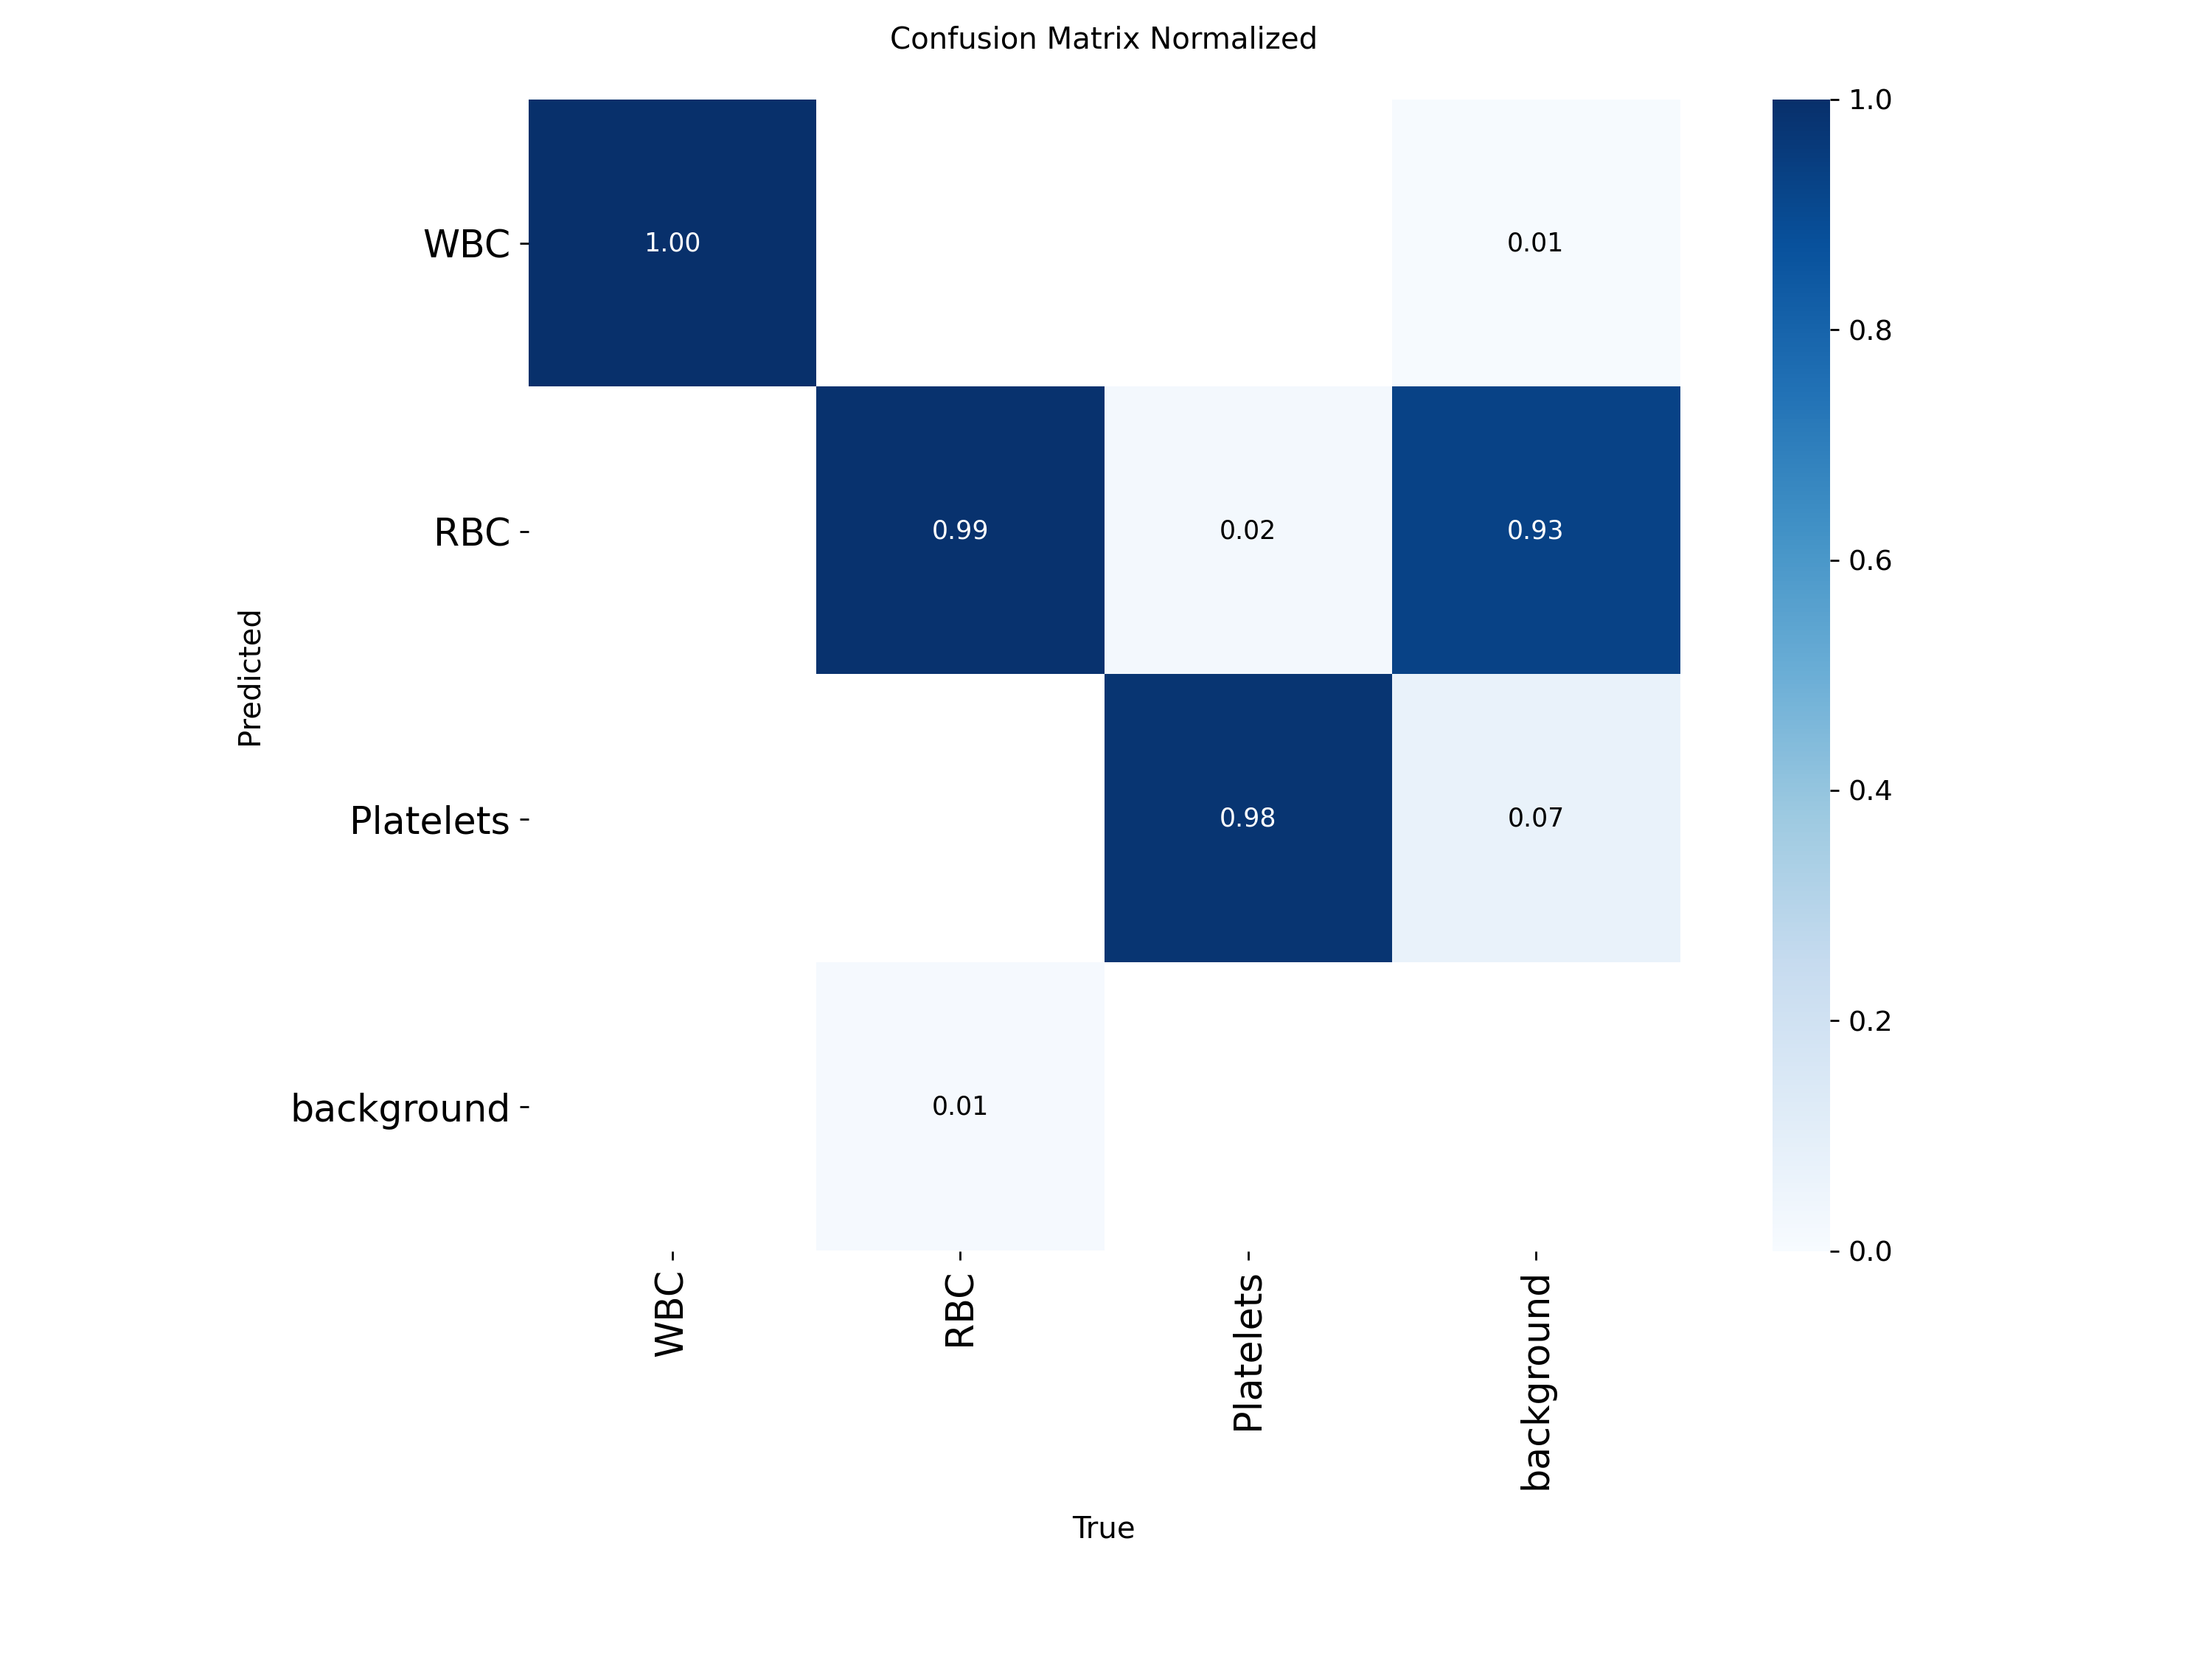
\includegraphics[width=\textwidth]{figures/stage1_results_confusion_matrix.png}
\caption{Normalised confusion matrix.}
\end{subfigure}\\[6pt]
\begin{subfigure}[t]{\textwidth}\centering
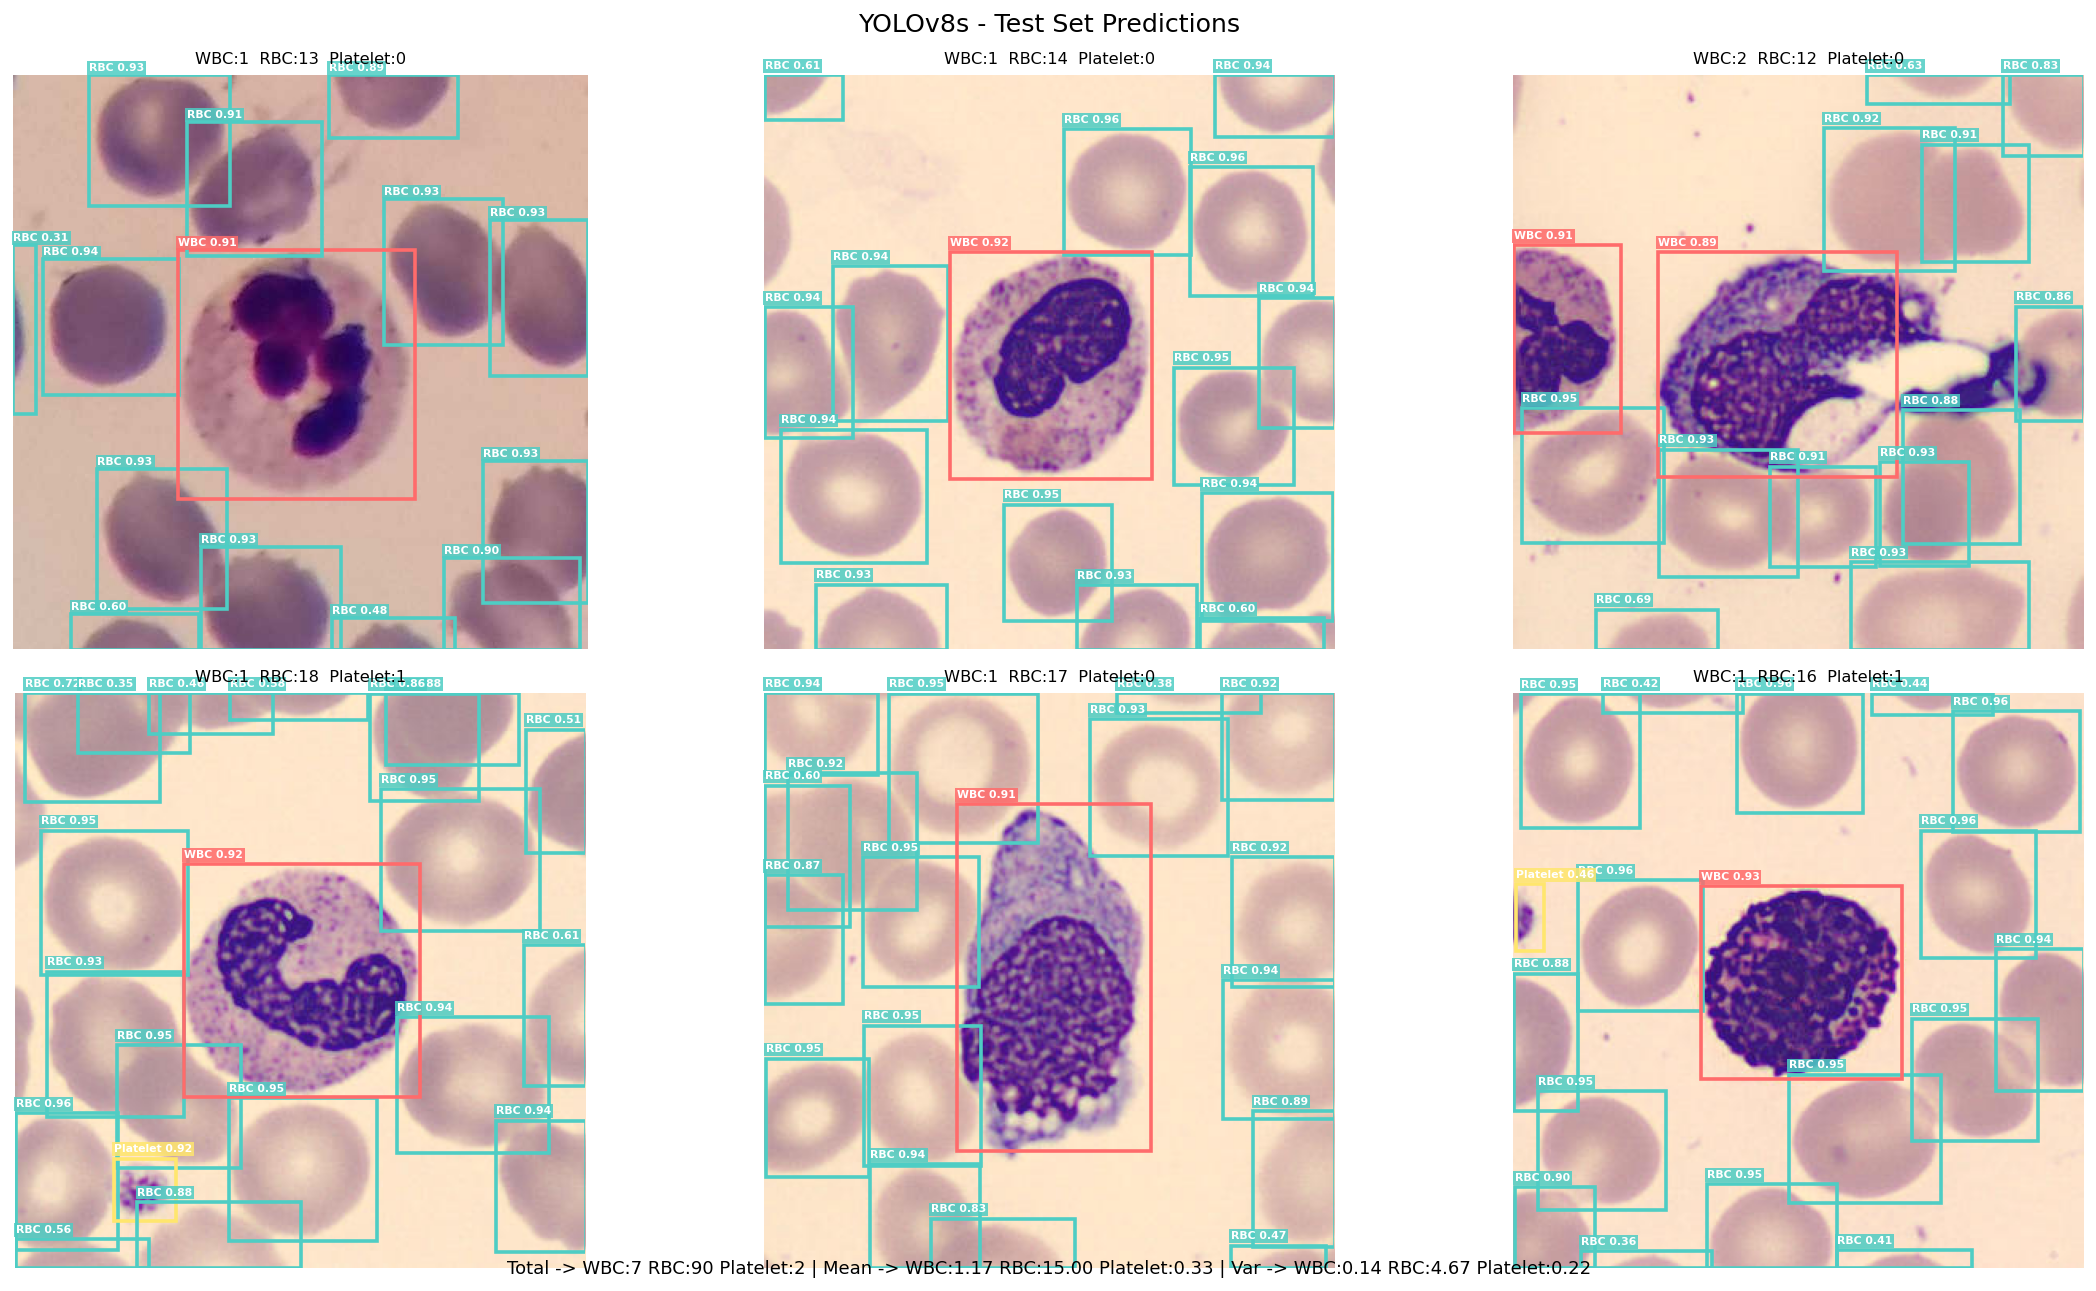
\includegraphics[width=0.9\textwidth]{figures/stage1_results_predictions.png}
\caption{Predictions on test images.}
\end{subfigure}
\caption{Detection results on the TXL-PBC test split.}
\label{fig:det}
\end{figure}

\begin{figure}[H]
\centering
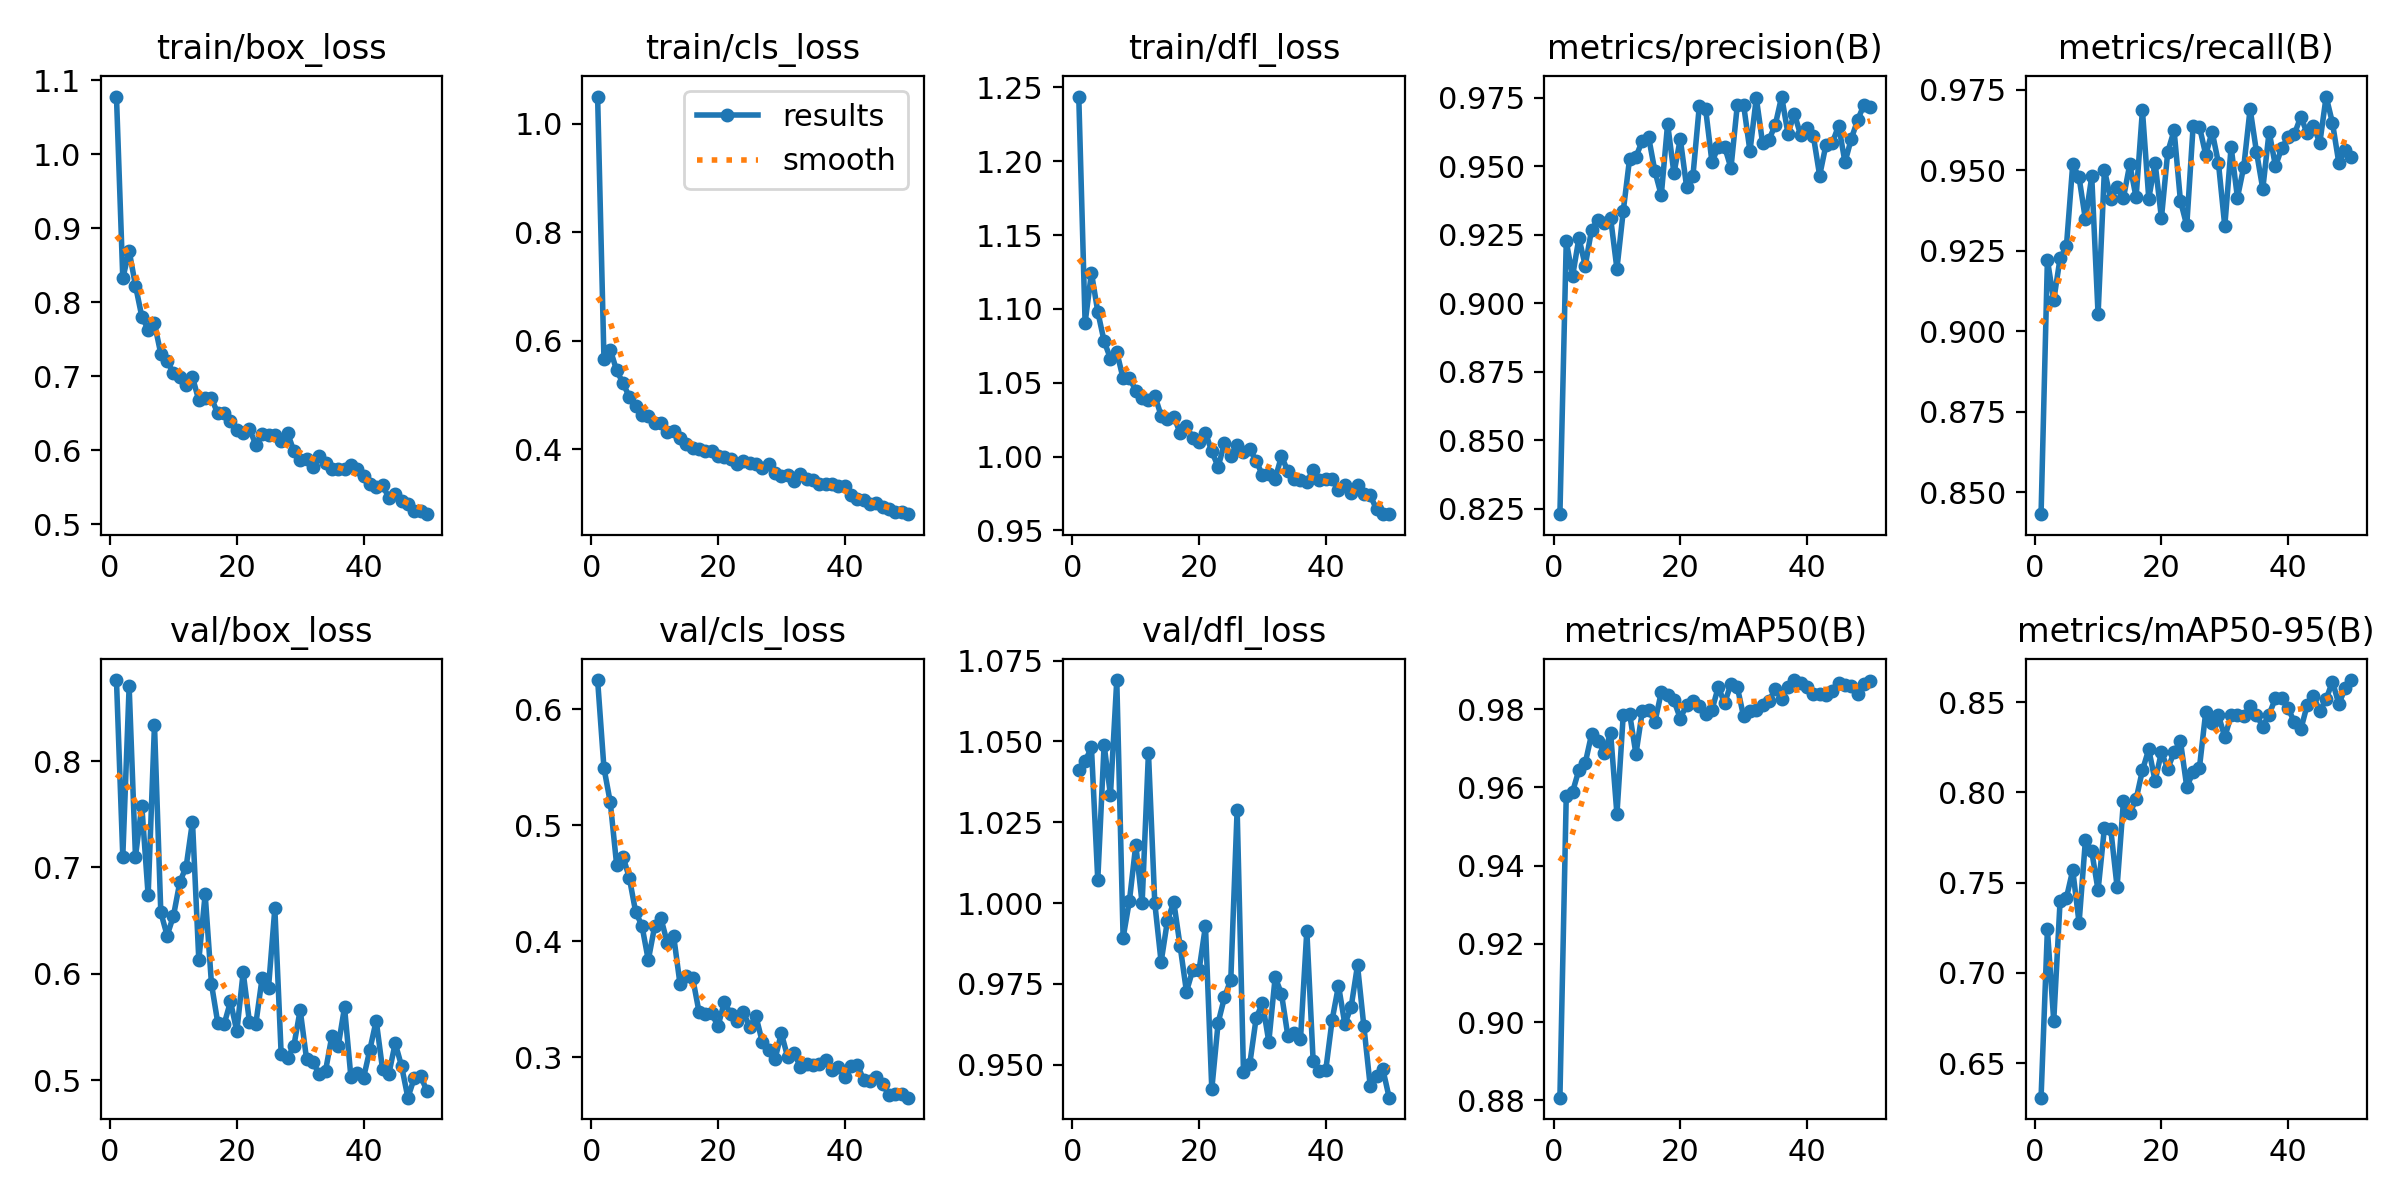
\includegraphics[width=\textwidth]{figures/stage1_results_training_curves.png}
\caption{YOLOv8s training curves over 50 epochs: training and validation box, class and distribution-focal losses (left three columns) and validation precision, recall, mAP@0.50 and mAP@0.50:0.95 (right).}
\label{fig:yolo-curves}
\end{figure}

\subsection{Stage 2: classification and uncertainty results}

The saved EfficientNet-B0 checkpoint reached a top-1 accuracy of \textbf{99.44\,\%} on the 3{,}419 PBC test images (macro-averaged F1 0.99). Per-class results are in Table~\ref{tab:cls} and the confusion matrix in Figure~\ref{fig:cls}. The only class below 0.99 recall is the immature granulocyte (0.98), whose errors go to neutrophils (0.02) and erythroblasts (0.01). This is morphologically plausible: immature granulocytes are transitional forms between myeloid precursors and mature neutrophils, and the boundary is also difficult for human reviewers. It is exactly the kind of case in which an uncertainty estimate is useful.

Freezing the backbone limited Phase~1 to a best monitored accuracy of 88.97\,\%; unfreezing it in Phase~2 raised this to 98.65\,\% within eight epochs, showing that adapting the pre-trained features is essential for fine-grained cell morphology. The final evaluation of the saved checkpoint, in a later notebook cell, gave 99.44\,\% on the same images; the difference between the two numbers was not investigated and suggests that the saved checkpoint is not exactly the one monitored in the displayed training log. Together with the caveat in Section~\ref{sec:method} --- the test images were also used for model selection --- this means that 99.44\,\% should be read as an optimistic estimate.

\begin{table}[H]
\centering
\caption{Per-class results of EfficientNet-B0 on the PBC test split (scikit-learn classification report).}
\label{tab:cls}
\small
\begin{tabular}{lcccr}
\toprule
\textbf{Class} & \textbf{Precision} & \textbf{Recall} & \textbf{F1} & \textbf{Support} \\
\midrule
Basophil & 1.00 & 1.00 & 1.00 & 237 \\
Eosinophil & 1.00 & 1.00 & 1.00 & 620 \\
Erythroblast & 0.98 & 1.00 & 0.99 & 309 \\
Immature granulocyte & 1.00 & 0.98 & 0.99 & 598 \\
Lymphocyte & 0.99 & 1.00 & 0.99 & 256 \\
Monocyte & 1.00 & 0.99 & 1.00 & 286 \\
Neutrophil & 0.98 & 1.00 & 0.99 & 649 \\
Platelet & 1.00 & 1.00 & 1.00 & 464 \\
\midrule
\textbf{Accuracy} & \multicolumn{3}{c}{\textbf{0.9944}} & 3{,}419 \\
\bottomrule
\end{tabular}
\end{table}

\begin{figure}[H]
\centering
\begin{subfigure}[t]{0.66\textwidth}\centering
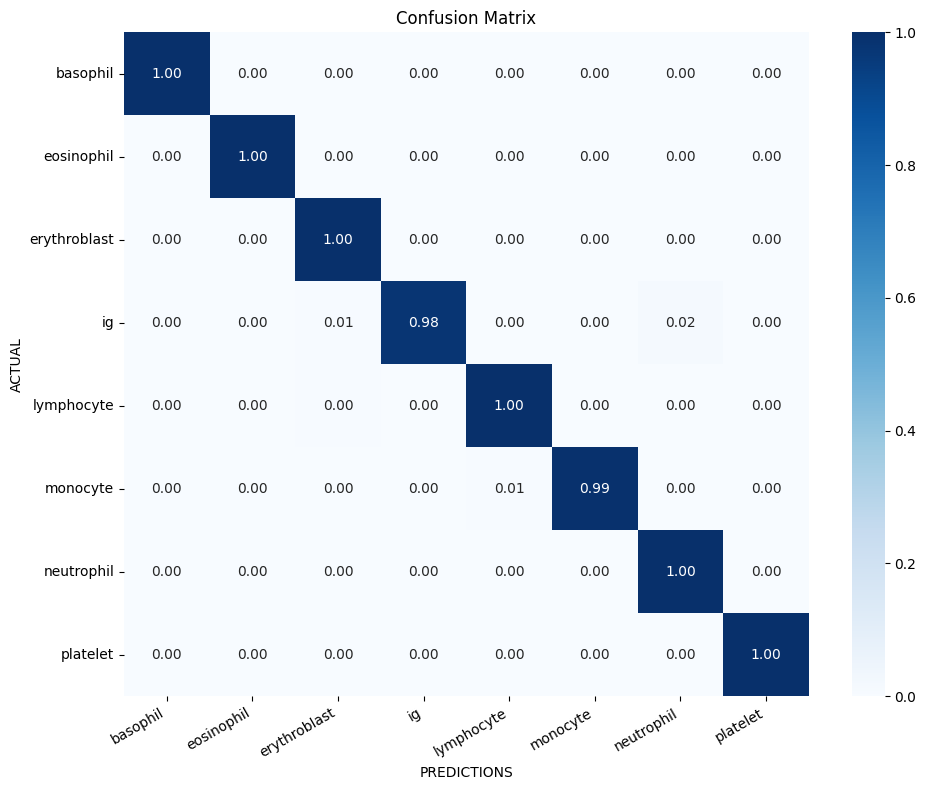
\includegraphics[width=\textwidth]{figures/stage2_embedded_confusion_matrix_test.png}
\caption{Normalised confusion matrix of the saved checkpoint.}
\end{subfigure}\\[6pt]
\begin{subfigure}[t]{\textwidth}\centering
\includegraphics[width=\textwidth]{figures/effnet_training_curves.pdf}
\caption{Loss and accuracy over both training phases, re-plotted from the notebook's training log. The ``monitored'' curve was computed on the test partition (see the caveat in Section~\ref{sec:method}).}
\end{subfigure}
\caption{Classification results on the PBC test split.}
\label{fig:cls}
\end{figure}

\begin{figure}[H]
\centering
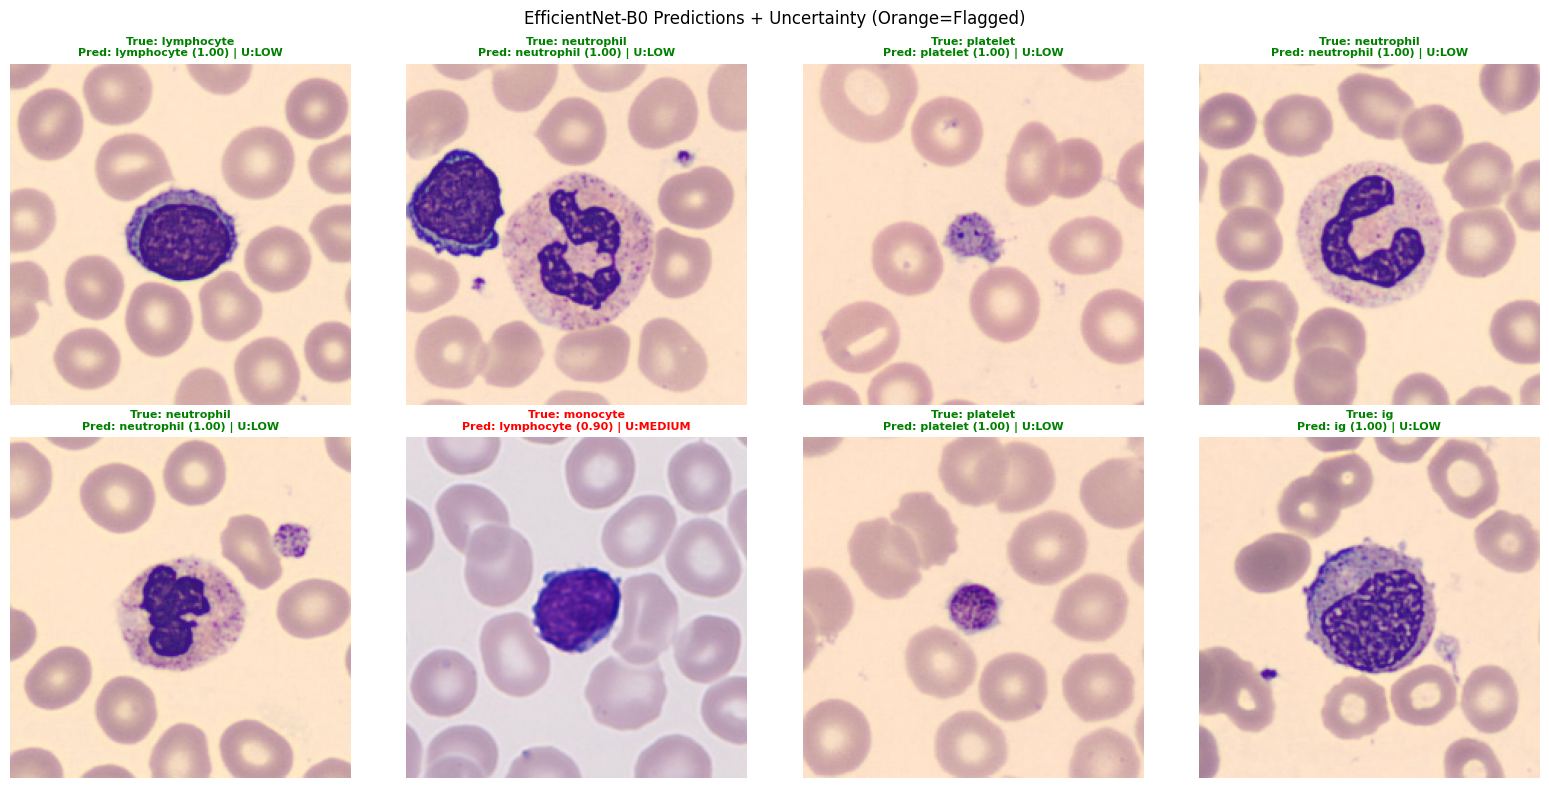
\includegraphics[width=0.9\textwidth,height=7cm,keepaspectratio]{figures/stage2_embedded_mc_dropout_uncertainty_demo.png}
\caption{MC-Dropout predictions on eight test images. The seven correct predictions receive the uncertainty level LOW; the one error (a monocyte predicted as a lymphocyte with confidence 0.90, red title) receives MEDIUM. MEDIUM is not flagged, so this error would not by itself trigger expert review.}
\label{fig:mc}
\end{figure}

\paragraph{An example of domain shift.} The PBC images used for training come from a single analyser with standardised staining. Figure~\ref{fig:shift} shows the combined Stage~1 + Stage~2 output on an image from a different source, produced in the Stage-3 notebook. The white cell has a segmented nucleus and granular cytoplasm, the appearance of a mature granulocyte, yet the classifier labelled it \emph{erythroblast} with a probability of 0.90. This single example does not measure the size of the problem, but it illustrates why the benchmark accuracy should not be expected to transfer unchanged to smears from other laboratories.

\begin{figure}[H]
\centering
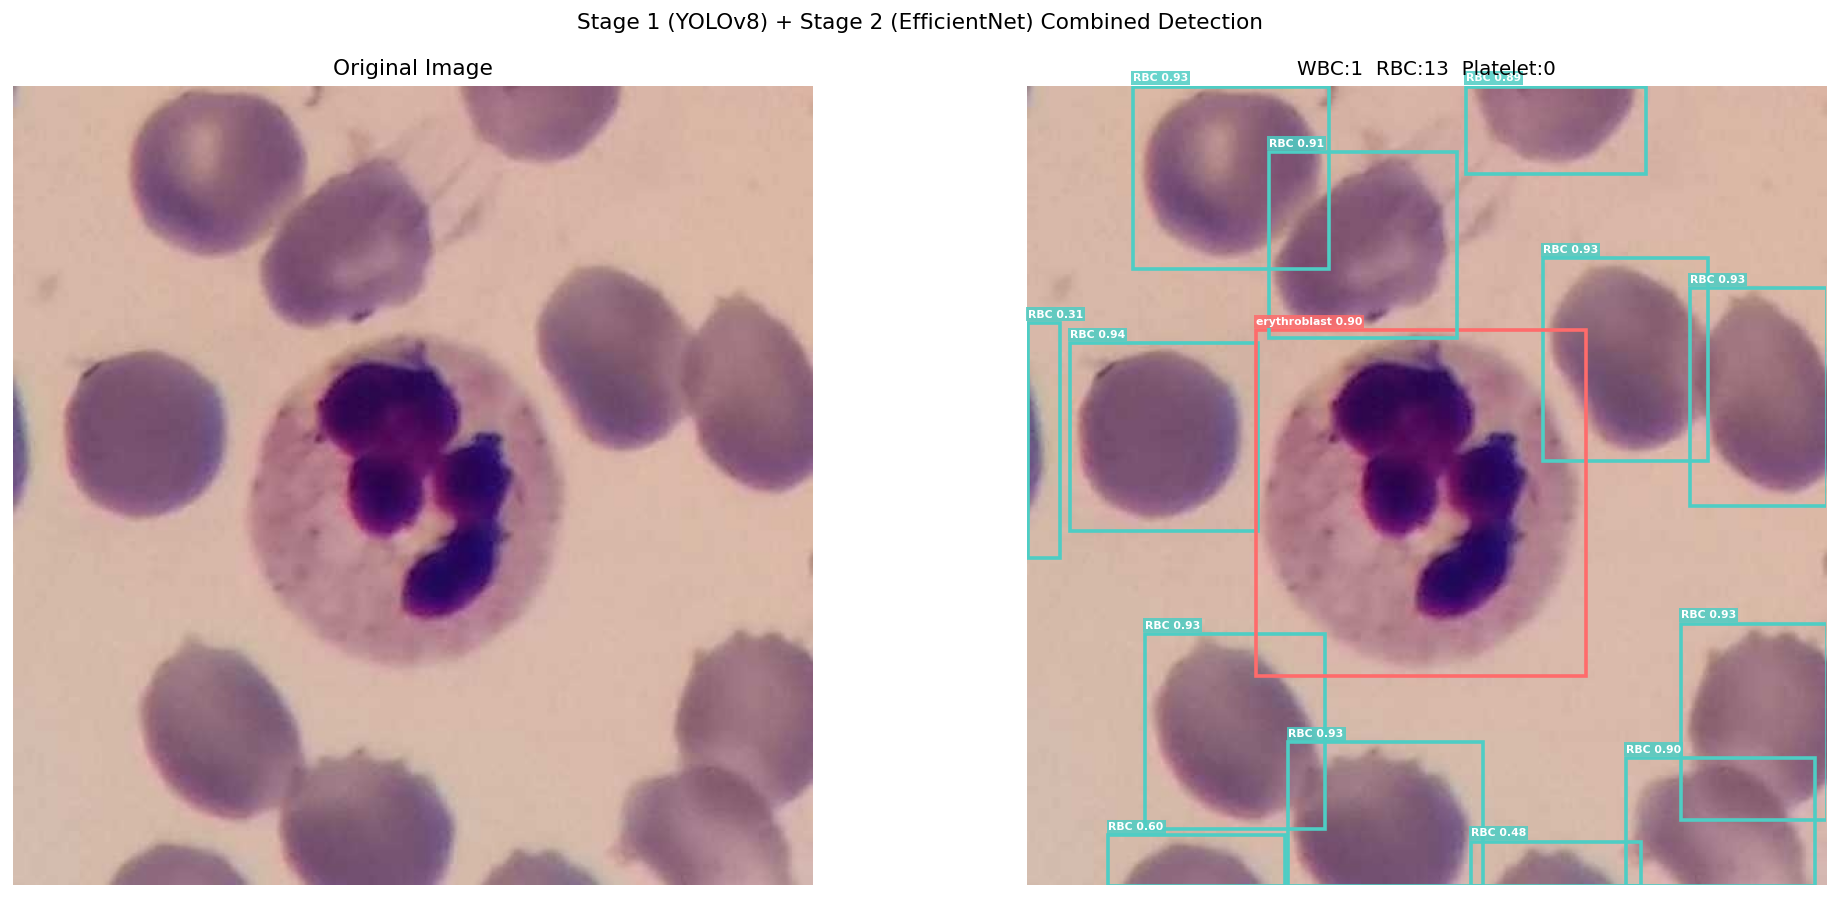
\includegraphics[width=0.9\textwidth]{figures/stage3_results_pipeline_output.png}
\caption{Stage 1 + Stage 2 output on an image from outside the training distribution: 13 red cells and one white cell were detected; the white cell, which appears to be a segmented granulocyte, was classified as \emph{erythroblast} (0.90). (This notebook run used a lower detection threshold than the 0.50 of the final system, so some low-confidence red-cell boxes are shown.)}
\label{fig:shift}
\end{figure}

No calibration study was performed: the thesis does not report whether cells marked HIGH uncertainty are more often misclassified. MC-Dropout is therefore used as a practical signal that makes difficult cells visible, not as a validated error predictor.

\subsection{Quantitative evaluation of the domain expert}\label{sec:res-de}

Table~\ref{tab:de} and Figure~\ref{fig:de} summarise the comparison of the base model, the fine-tuned model and GPT-4o.

\begin{table}[H]
\centering
\caption{Domain-expert evaluation. In-domain metrics are means over 100 held-out textbook questions; MedMCQA accuracy is over 100 hematology-related exam questions (not run for GPT-4o). Best value per column in bold.}
\label{tab:de}
\small
\begin{tabular}{lccccc}
\toprule
 & \multicolumn{4}{c}{\textbf{In-domain held-out questions}} & \textbf{External} \\
\cmidrule(lr){2-5}\cmidrule(lr){6-6}
\textbf{System} & \textbf{Sem.\ sim.} & \textbf{ROUGE-L} & \textbf{Source marker} & \textbf{Words} & \textbf{MedMCQA} \\
\midrule
Llama-3.1-8B (base) & 0.752 & 0.161 & 7\,\% & 158.5 & 56\,\% \\
Llama-3.1-8B + QLoRA (ours) & \textbf{0.831} & \textbf{0.433} & 100\,\% & 39.4 & \textbf{57\,\%} \\
GPT-4o (reference) & 0.774 & 0.181 & 88\,\% & 159.9 & -- \\
\midrule
Reference answers & -- & -- & 100\,\% & 39.2 & -- \\
\bottomrule
\end{tabular}
\end{table}

\begin{figure}[H]
\centering
\includegraphics[width=\textwidth]{figures/domain_expert_results.pdf}
\caption{Comparison of the three systems: (a) semantic similarity and (b) ROUGE-L F1 against the textbook reference answers on 100 held-out questions; (c) accuracy on 100 hematology-related MedMCQA questions, with the 25\,\% chance level.}
\label{fig:de}
\end{figure}

\paragraph{In-domain questions.} Fine-tuning brought the model's answers much closer to the textbook reference answers. ROUGE-L rose from 0.161 to 0.433; the paired bootstrap 95\,\% confidence interval of the improvement is $[0.252,\ 0.293]$, and the fine-tuned model scored higher than the base model on \emph{every one} of the 100 questions. Semantic similarity rose from 0.752 to 0.831. On both measures the fine-tuned 8-billion-parameter model also exceeded GPT-4o (ROUGE-L difference $+0.252$, 95\,\% CI $[0.234,\ 0.273]$). Its answers are about four times shorter than those of the other two systems (39 vs.\ 159 words) and match the length of the reference answers (39 words).

These numbers must be read carefully. The reference answers were written by a GPT model from the textbook passages, in a particular concise style, and the fine-tuned model was trained on 1{,}890 answers in exactly that style. Part of the gain is therefore a gain in \emph{form}: length, wording and structure. ROUGE-L rewards this strongly; semantic similarity, which is less sensitive to wording, shows a smaller but still clear gain. GPT-4o's lower scores do not mean that its answers are less correct --- it writes longer, more general explanations that overlap less with the short reference text.

\paragraph{External questions.} On the MedMCQA questions the fine-tuned model answered 57 of 100 correctly and the base model 56. The two models disagreed on 21 questions (base correct only: 10; fine-tuned correct only: 11), and the exact McNemar test gives $p = 1.0$: there is no evidence of a difference. Fine-tuning on 1{,}890 textbook pairs neither improved nor damaged the model's general hematology knowledge. (Both models are well above the 25\,\% chance level; three of the base model's answers could not be parsed as a letter and count as wrong.)

\paragraph{Interpretation.} Together, the two results give a clear picture: \emph{QLoRA fine-tuning taught the model how the domain expert should answer --- concisely, in the textbook's terminology and with a source line --- but it did not teach it new medical knowledge.} This agrees with the literature, which finds that retrieval is more effective than fine-tuning for injecting knowledge \cite{ovadia2024}, and it supports the design choice of building the runtime expert around retrieval and tools.

\subsection{Qualitative analysis: citations and errors}

\paragraph{Invented citations in the base model.} No source was given to the models, yet the base Llama model named a specific textbook, author or edition in \textbf{52 of the 100} in-domain answers. Typical openings were:

\begin{quote}\small
``According to the textbook \emph{`Hematology: A Very Short Introduction'} by Valerie Higgs [1] \ldots'' \\
``According to the textbook \emph{`Hematopathology'} by Knowles, 2nd edition, [Reference 1] \ldots''
\end{quote}

The attributions are fabricated --- the model was never shown these books, and in several answers the same title is attributed to different authors --- but they look convincing. This is the failure mode described by Walters and Wilder for ChatGPT \cite{walters2023}, and it is caused here by the system prompt, which asks the model to ``cite'' a ``provided textbook reference'' that is not there. Neither the fine-tuned model nor GPT-4o named an invented book. GPT-4o, however, inserted a bare ``[Reference~1]'' marker in 32 answers, pointing to a reference that did not exist --- a milder form of the same behaviour.

\paragraph{Uniform source lines in the fine-tuned model.} The fine-tuned model ended \emph{every} answer with a source line (100\,\% in Table~\ref{tab:de}), naming the first textbook in 92 answers and the second in 8. It usually chose the right book --- five of the seven questions from the second book were labelled correctly --- which shows that it learned which topics belong to which book. But the line is learned format, not provenance: the model attaches it to correct and incorrect answers alike. Examples of incorrect answers that carry the source line are:

\begin{itemize}
  \item \emph{Pure red cell aplasia}: the model expects ``macrocytic red cells'', whereas the reference answer describes a normocytic normochromic anaemia with reticulocytopenia.
  \item \emph{Hypertransfusion in thalassaemia}: the model states a target haemoglobin ``above 14\,g/dl''; the reference answer gives 9.5--10\,g/dl.
  \item \emph{Myeloblast vs.\ lymphoblast} (qualitative question): the model describes the myeloblast as having ``coarse nuclear chromatin'' and ``2--3 large, bright blue, specific granules'', which is incorrect --- myeloblasts typically have fine chromatin and few or no granules.
\end{itemize}

The fine-tuned model therefore looks more authoritative than the base model while being no more knowledgeable. For a domain expert this is an important and somewhat uncomfortable finding: \textbf{a citation produced by a language model is not evidence}. A citation is only useful if it points to a passage that was actually retrieved and can be opened, as in the RAG agent, where every \code{[Reference N]} corresponds to a logged tool result.

\paragraph{Clinical scenarios.} Table~\ref{tab:qual} summarises the answers to the five hand-written clinical questions. Both models recognise the typical patterns (neutrophilic leukocytosis with toxic granulation suggests infection or inflammation; a microcytic anaemia with target cells suggests a hemoglobinopathy). The fine-tuned model is shorter and more decisive; the base model is longer, lists more possibilities, and often decorates its answer with invented reference numbers.

\begin{table}[H]
\centering
\caption{Condensed answers to the five clinical questions (full answers in \code{evaluation\_report.json}).}
\label{tab:qual}
\footnotesize
\begin{tabularx}{\textwidth}{>{\raggedright\arraybackslash}p{3.3cm} X X}
\toprule
\textbf{Question} & \textbf{Base model} & \textbf{Fine-tuned model} \\
\midrule
78\,\% neutrophils, toxic granulation, WBC $18 \times 10^9$/L & Leukemoid reaction or severe (bacterial) infection; long explanation & ``Neutrophilic leucocytosis with toxic granules'', suggests infection/inflammation \\
Only 2 WBCs classified (1 IG, 1 monocyte) & Classification incomplete; the differential is not representative & ``Differential unsatisfactory'' because far too few cells were counted \\
Hb 9.1\,g/dL, MCV 68\,fL, target cells & Thalassaemia, HbC, HbE, sickle cell disease, iron deficiency; Hb electrophoresis & Thalassaemia trait, sickle cell trait, Hb Lepore; solubility test for HbS (omits iron deficiency) \\
Myeloblast vs.\ lymphoblast & Mostly correct list of features & Contains factual errors (see text) \\
Platelets $90 \times 10^9$/L --- always true thrombocytopenia? & Attributes the answer to an invented textbook & ``No'' --- counts can be falsely low; correct in essence \\
\bottomrule
\end{tabularx}
\end{table}

Notably, both models --- when asked directly --- recognised that a differential based on two cells is not meaningful. As the next sections show, the full system did \emph{not} make this judgement when the same situation arose in a real run.

\subsection{End-to-end case study: an over-interpreted differential}\label{sec:case}

The saved result files in the repository contain one complete run of the system in its default configuration (GPT-4o agent) on an uploaded $640 \times 480$ smear image. It is analysed here in detail because it shows both the strengths of the design and a failure that the safety logic did not catch.

\paragraph{What the system did.} Stage~1 detected 17 red cells and \textbf{2 white cells}. Stage~2 classified one white cell as an immature granulocyte (confidence 0.955, entropy 0.216) and the other as a monocyte (confidence 0.972, entropy 0.146); both received the uncertainty level LOW, so no cell was flagged. The agent then made five tool calls: it looked up the reference ranges of immature granulocytes (0--0.5\,\%) and monocytes (2--8\,\%), read the uncertainty summary, and searched the knowledge base for ``causes of increased immature granulocytes'' and ``causes of monocytosis''. Its final report stated:

\begin{quote}\small
``The peripheral blood smear shows a significant increase in immature granulocytes (50\,\%) and monocytes (50\,\%), which is highly abnormal. [\ldots] Immature granulocytes (IG) at 50\,\%, significantly above the normal range of 0--0.5\,\% [Reference 6].'' --- Recommendation: ``Consider bone marrow biopsy if clinically indicated.'' --- \code{confidence\_assessment}: HIGH, \code{requires\_expert\_review}: \textbf{false}.
\end{quote}

\paragraph{What went wrong.} Three problems can be identified.
\begin{enumerate}
  \item \textbf{The sample was far too small.} A differential expresses each cell type as a percentage of the white cells counted. Routine manual differentials count at least 100 cells, and the reference method of CLSI H20-A2 counts several hundred \cite{clsi2007h20}. Two cells cannot establish any percentage; ``50\,\% immature granulocytes'' is an artefact of dividing by two. The system prompt told the agent that the counts are per microscope field, but it did not tell it to check the number of cells, and nothing in the code did.
  \item \textbf{A citation was misattributed.} The retrieved chunk labelled Reference~6 is about hypersegmented neutrophils in megaloblastic anaemia. The range 0--0.5\,\% actually came from the reference-range tool. The claim was correct, but its citation pointed to the wrong evidence --- the kind of error that only becomes visible because the tool trace is recorded.
  \item \textbf{The review flag stayed false.} Both cells had low MC-Dropout uncertainty, so the deterministic rule did not fire, and the model itself set the flag to false while recommending a bone-marrow biopsy. The uncertainty of the \emph{individual cells} was low; what was uncertain was the \emph{differential as a whole}, and the rule did not measure that.
\end{enumerate}

\paragraph{Lessons.} The case shows that the design choices of the thesis --- a recorded tool trace, retrieved passages that can be checked, uncertainty passed forward --- make such failures \emph{detectable}: every step above could be reconstructed from the saved output. But it also shows that per-cell uncertainty is not enough. The fix is simple and deterministic, and it has since been implemented (Section~\ref{sec:safety}): whenever fewer than a minimum number of white cells (by default 100, which in practice requires several fields of view) have been classified, the pipeline forces \code{requires\_expert\_review} to true and adds an \code{INSUFFICIENT\_CELL\_COUNT} flag, and the reasoners are told not to interpret the percentages. Applied to this case (2 cells), the rule sets the flag to true; this is covered by an automated test. The case study run itself was made before the rule existed and was not repeated. Interestingly, both language models answered correctly when asked about a two-cell differential directly (Table~\ref{tab:qual}); in the agent, the structured prompt and the tool outputs led the model to compute and interpret percentages instead. This is a strong argument for putting such domain rules into code rather than relying on the model's judgement.

\subsection{Discussion of the research questions}

\paragraph{RQ1 --- blood image classification.} Standard vision models provide strong evidence on the benchmark data: mAP@0.50 = 0.985 for detection with perfect white-cell recall, and 99.44\,\% (optimistic) classification accuracy, each classified cell carrying an uncertainty level and a Grad-CAM map. How well this transfers to smears from other laboratories was not tested.

\paragraph{RQ2 --- building the domain expert with RAG.} A general LLM was turned into a hematology expert by combining a curated textbook knowledge base, domain tools and a structured output format. The resulting agent produces interpretations with retrievable citations and a complete, auditable tool trace (Figures~\ref{fig:ui-a}--\ref{fig:ui-b}). The case study shows that this makes errors visible but does not prevent them; domain rules such as a minimum cell count must be enforced in code.

\paragraph{RQ3 --- domain fine-tuning.} QLoRA fine-tuning of Llama-3.1-8B for under an hour on a free GPU produced a model whose answers match textbook reference answers much better than those of the base model and even of GPT-4o (ROUGE-L 0.433 vs.\ 0.161 and 0.181), and which no longer invents book references. It did not improve accuracy on external exam questions (57\,\% vs.\ 56\,\%, not significant), and it learned to attach a source line regardless of correctness. Fine-tuning is therefore suitable for adapting the \emph{behaviour} of an open, self-hostable expert, but it must be combined with retrieval to supply knowledge and real provenance.

\paragraph{RQ4 --- safety and auditability.} The system passes all safety-relevant information forward and forces expert review when any cell is uncertain. The case study showed the limits of the original rule: it reacted to uncertain \emph{cells}, not to an unreliable \emph{differential}. A minimum-cell rule was therefore added. Auditability worked as intended --- the misattributed citation and the faulty reasoning could be traced step by step.

\subsection{Limitations and threats to validity}

\begin{itemize}
  \item \textbf{Synthetic reference answers.} The in-domain test answers were generated by a GPT model from the textbook, not written by hematologists. They may contain errors, and they favour a model trained on the same style. Some questions refer to ``the passage'', an artefact of the generation.
  \item \textbf{Grouping assumption in the split.} The chunk-level split assumes that consecutive records come from the same chunk, as written by the generation script; the records themselves do not store a chunk identifier.
  \item \textbf{Small, noisy external test.} The MedMCQA subset has 100 questions, about a quarter of which are only loosely related to hematology; small differences cannot be detected with this sample size.
  \item \textbf{No human or LLM-judge ratings.} Correctness was assessed with automatic similarity measures and by hand for a few answers. The planned LLM-as-judge step failed, and no clinician evaluated the answers.
  \item \textbf{Training format of the fine-tuned model.} The training examples contain no retrieved passage, so the model was not trained to read and cite evidence. The fine-tuned model was evaluated stand-alone, not inside the agent.
  \item \textbf{Classifier evaluation.} The EfficientNet test set was also used for checkpoint selection, the split is image-level rather than donor-level, and the saved checkpoint's accuracy (99.44\,\%) differs from the monitored training accuracy (98.65\,\%) without explanation. (A mismatch in the inference code, which re-created the second dropout layer with $p = 0.2$ instead of the $p = 0.3$ used in training, was found during this work and corrected; the case-study run predates the correction.)
  \item \textbf{No external validation of the vision stages.} Both vision datasets were recorded under controlled conditions; smears from other microscopes, stains or laboratories may reduce performance substantially.
  \item \textbf{Uncertainty thresholds and review rule} were set by hand and are not calibrated against error rates.
  \item \textbf{Copyright of the knowledge base.} The textbooks are copyrighted and cannot be redistributed, which limits exact reproduction of the knowledge base by others.
\end{itemize}

\clearpage

\section{Conclusion}\label{sec:conclusion}

On the topic of developing a domain expert with a large language model like ChatGPT, this thesis built a hybrid multimodal lab assistant for peripheral blood smears, in which deep-learning models classify the cells in the image and a domain-expert LLM, grounded in hematology textbooks through RAG, interprets the findings. The domain expert was built in two complementary forms. The first is a GPT-4o agent that answers from a retrieval-grounded hematology knowledge base of 1{,}049 textbook passages, uses domain tools for reference ranges, cell counts and uncertainty, and returns a structured interpretation with a complete tool trace. The second is an open-weight Llama-3.1-8B model, adapted to the domain with QLoRA in under an hour on a free GPU, which can run on local hardware without a commercial API. Two image-analysis stages supply the case evidence: a YOLOv8s detector (mAP@0.50 = 0.985) and an EfficientNet-B0 classifier (98.60\,\% accuracy on a clean held-out test set), whose predictions carry Monte Carlo Dropout uncertainty --- which identifies misclassified cells with an AUROC of 0.97 --- and Grad-CAM saliency.

The central finding concerns what each technique contributes to a domain expert. Fine-tuning changed \emph{how} the model answers: its answers became concise and textbook-like, matching held-out reference answers far better than those of the base model and of GPT-4o, and it stopped inventing book references. It did not change \emph{what} the model knows: an LLM judge found no gain in clinical correctness, accuracy on external exam questions was unchanged, and the model attached a source line to incorrect answers as confidently as to correct ones. A citation generated by a language model is therefore not evidence. Knowledge and provenance must come from retrieval of real, inspectable passages, and the decision to involve a human must be taken by explicit rules. The end-to-end case study confirmed both points: the recorded tool trace made every error traceable, but the expert still turned a two-cell sample into a ``highly abnormal'' differential, because at the time no rule checked the number of cells --- a rule that has since been added.

The practical answer to the thesis topic is thus a layered design: \emph{fine-tuning for behaviour, retrieval for knowledge, tools for case data, and deterministic rules for safety}. The system is a research prototype. It has not been validated clinically, its vision models have not been tested on data from other laboratories, and its expert answers were evaluated with automatic measures rather than by hematologists.

\subsection{What was not achieved}

Several aims were met only partly, and they are stated here explicitly.

\begin{itemize}
  \item \textbf{The fine-tuned open model did not become a better expert in substance.} The hope that QLoRA fine-tuning would make Llama-3.1-8B more knowledgeable was not confirmed: clinical correctness (LLM judge) and exam accuracy were unchanged, and the model remained clearly less correct than GPT-4o. It is therefore not yet a replacement for the hosted model, only a self-hostable starting point.
  \item \textbf{The fine-tuned model was not evaluated inside the full assistant.} It was tested stand-alone, without retrieved passages; the combination of the open model with RAG and tools --- the configuration that the results suggest --- was not run end-to-end.
  \item \textbf{The end-to-end evaluation is a single case.} Only one complete run of the assistant was analysed in depth. It exposed a real failure (the two-cell differential), which led to a new safety rule, but a systematic evaluation over many smears, ideally rated by hematologists, is still missing.
  \item \textbf{The first classifier evaluation was flawed.} The original training run selected its checkpoint on the test images. This was detected during the work and corrected by retraining; the corrected accuracy (98.60\,\%) is 0.84 points lower than the originally reported figure.
  \item \textbf{Generalisation was not measured.} All image results come from curated benchmark data. A single example from another source was misclassified, which suggests that performance on smears from other laboratories may be lower.
  \item \textbf{The optional CBC input was implemented but not evaluated.}
\end{itemize}

None of these points invalidates the main conclusion; rather, they define the limits within which it holds.

\subsection{Future work}

\begin{enumerate}
  \item \textbf{Multi-field analysis.} The new minimum-cell rule means that a single field of view will almost always be flagged. Aggregating the cells of many fields (or a whole-slide image) into one differential is the natural next step towards a clinically meaningful count.
  \item \textbf{Retrieval-aware fine-tuning.} Train the open model on examples that include the retrieved passage, so that it learns to answer from and cite the evidence it is given, and evaluate it inside the agent against GPT-4o on the same cases.
  \item \textbf{Expert evaluation.} Have hematologists or medical students rate a sample of answers for correctness and faithfulness, and compare their ratings with those of the LLM judge.
  \item \textbf{Review threshold.} Decide with clinical users whether MEDIUM-uncertainty cells should also be flagged: on the test set this would catch 82\,\% instead of 51\,\% of the errors at a review rate of 4.8\,\% of cells.
  \item \textbf{External validation.} Test both vision models on smears from another source (e.g.\ Raabin-WBC or local data), ideally with a donor-level split, and repeat the calibration and error-detection analysis under this distribution shift, comparing MC-Dropout with deep ensembles.
  \item \textbf{Laboratory values.} Add a CBC input to the web interface and evaluate whether CBC values improve the interpretations.
\end{enumerate}


\clearpage
\phantomsection
\addcontentsline{toc}{section}{\numberline{8}Bibliography}
\renewcommand{\refname}{8\hspace{1em}Bibliography}
\bibliographystyle{unsrtnat}
{\small
\bibliography{references}}

\clearpage
\setcounter{section}{8}
\section{Appendix}

\subsection*{A.\quad Reproducing the results}
\addcontentsline{toc}{subsection}{A.\quad Reproducing the results}

\begin{table}[H]
\centering
\footnotesize
\begin{tabularx}{\textwidth}{>{\raggedright\arraybackslash}p{3.6cm} >{\raggedright\arraybackslash}X}
\toprule
\textbf{Result} & \textbf{Where to find or re-run it} \\
\midrule
Domain-expert training and evaluation & \path{Notebooks/Domain_Expert_Finetune/domain_expert_evaluation.ipynb} (Colab T4, $\approx$1.5 h); outputs in \path{results/domain_expert/} \\
Q\&A dataset generation & \path{scripts/build_finetune_dataset.py}; data in \path{data/finetune/train.jsonl} \\
Detector training and test metrics & \path{Notebooks/YOLOv8_detection/YOLOv8_on_TBL_PBC_dataset.ipynb} \\
Classifier training and test metrics & \path{Notebooks/Efficientnet_classification/Efficientnet_classification.ipynb} \\
Case-study run & \path{results/stage1_detection.json}, \path{stage2_classification.json}, \path{stage3_reasoning.json} \\
Running the full system & \code{python main.py analyze <image>}, or \code{start.ps1} for the web interface \\
All runtime settings & \code{config.yaml} \\
\bottomrule
\end{tabularx}
\end{table}

\subsection*{B.\quad Main configuration values}
\addcontentsline{toc}{subsection}{B.\quad Main configuration values}

\begin{table}[H]
\centering
\small
\begin{tabular}{lll}
\toprule
\textbf{Key} & \textbf{Value} & \textbf{Meaning} \\
\midrule
\code{detection.confidence\_threshold} & 0.50 & minimum box confidence \\
\code{classification.mc\_dropout\_passes} & 20 & $T$ in MC-Dropout \\
\code{classification.uncertainty.low} & conf.\ $\ge$ 0.85, entropy $<$ 0.3 & LOW level \\
\code{classification.uncertainty.medium} & conf.\ $\ge$ 0.65, entropy $<$ 0.6 & MEDIUM level \\
\code{rag.chunking.chunk\_size / overlap} & 200 / 40 words & text chunking \\
\code{rag.embedding.model\_name} & \code{all-MiniLM-L6-v2} & embedding model \\
\code{rag.retrieval.top\_k} & 5 & chunks per query \\
\code{rag.internet.enabled} & false & web augmentation \\
\code{reasoning.mode} & agent & \code{agent} or \code{linear} \\
\code{reasoning.agent.max\_iterations} & 6 & agent step budget \\
\code{llm.model\_name / temperature} & gpt-4o / 0.1 & language model \\
\code{llm.safety.min\_wbc\_for\_differential} & 100 & minimum-cell rule \\
\bottomrule
\end{tabular}
\end{table}

\clearpage
\subsection*{C.\quad Output of the domain-expert agent (abridged)}
\addcontentsline{toc}{subsection}{C.\quad Output of the domain-expert agent (abridged)}

The complete output of the case-study run (Section~\ref{sec:case}), shortened:

\begin{lstlisting}
{
 "clinical_interpretation": "The peripheral blood smear shows a significant
    increase in immature granulocytes (50%) and monocytes (50%), which is
    highly abnormal. ...",
 "key_findings": [
    "Immature granulocytes (IG) at 50%, significantly above the normal
     range of 0-0.5% [Reference 6].", "..."],
 "differential_diagnoses": [
    "Infection or bone marrow stress [Reference 6] - ...", "..."],
 "recommendations": [
    "...", "Consider bone marrow biopsy if clinically indicated."],
 "safety_flags": [
    "High levels of immature granulocytes and monocytes warrant further
     investigation ..."],
 "confidence_assessment": "HIGH",
 "requires_expert_review": false,
 "reasoning_mode": "agent",
 "agent_trace": [
  {"type": "tool_call", "name": "lookup_lab_reference_ranges",
   "args": {"parameter": "ig"}},
  {"type": "tool_call", "name": "lookup_lab_reference_ranges",
   "args": {"parameter": "monocyte"}},
  {"type": "tool_call", "name": "get_uncertainty_summary", "args": {}},
  {"type": "tool_call", "name": "query_knowledge_base",
   "args": {"query": "causes of increased immature granulocytes"}},
  {"type": "tool_call", "name": "query_knowledge_base",
   "args": {"query": "causes of monocytosis"}},
  ... five tool results and the final message ...
 ]
}
\end{lstlisting}

\subsection*{D.\quad Declaration on the use of generative AI}
\addcontentsline{toc}{subsection}{D.\quad Declaration on the use of generative AI}

Generative AI tools were used in this work in three ways: (1) GPT-4o and a Llama-3.1 model are components of the system and are described as such; (2) an OpenAI GPT model generated the synthetic question--answer pairs used for fine-tuning and testing (Section~\ref{sec:qa-data}); and (3) AI assistants were used to help draft and refactor code and text. All design decisions, experiments, reported results and final wording are the author's responsibility, and all numbers in this thesis were taken from the saved outputs of the experiments.


\clearpage
\section*{Acknowledgment}
\addcontentsline{toc}{section}{Acknowledgment}
I would like to thank my supervisor, Dr.\ András Hajdu, for his guidance and patience throughout this project. I am grateful to the authors of the TXL-PBC, PBC and MedMCQA datasets for making their data openly available, and to the maintainers of Ultralytics, PyTorch, \code{timm}, Unsloth, Hugging Face Transformers, ChromaDB, LangChain/LangGraph, FastAPI and Vite, whose open-source work made this single-author project possible.

\end{document}
